\documentclass[12pt,reqno]{amsart}
\usepackage[pdfborder={0 0 0.5 [3 2]}, plainpages=false]{hyperref}%
\usepackage[left=1in,right=1in,top=1in,bottom=1in]{geometry}%
\usepackage[citation-order]{amsrefs}%
\usepackage{amsmath}
\usepackage{enumerate}
\usepackage{amssymb}                
\usepackage{amsfonts}
\usepackage{amsthm}
\usepackage{bbm}
\usepackage[table,xcdraw]{xcolor}
\usepackage{float}
\usepackage{mathtools}
\usepackage{cool}
\usepackage{booktabs}
\usepackage{graphicx,epsfig}

\usepackage[capitalize,nameinlink]{cleveref}
% Per SIAM Style Manual, "section" should be lowercase
\crefname{section}{section}{sections}
\crefname{subsection}{subsection}{subsections}
\Crefname{section}{Section}{Sections}
\Crefname{subsection}{Subsection}{Subsections}

% Per SIAM Style Manual, "Figure" should be spelled out in references
\Crefname{figure}{Figure}{Figures}

% Per SIAM Style Manual, don't say equation in front on an equation.
\crefformat{equation}{\textup{#2(#1)#3}}
\crefrangeformat{equation}{\textup{#3(#1)#4--#5(#2)#6}}
\crefmultiformat{equation}{\textup{#2(#1)#3}}{ and \textup{#2(#1)#3}}
{, \textup{#2(#1)#3}}{, and \textup{#2(#1)#3}}
\crefrangemultiformat{equation}{\textup{#3(#1)#4--#5(#2)#6}}%
{ and \textup{#3(#1)#4--#5(#2)#6}}{, \textup{#3(#1)#4--#5(#2)#6}}{, and \textup{#3(#1)#4--#5(#2)#6}}

% But spell it out at the beginning of a sentence.
\Crefformat{equation}{#2Equation~\textup{(#1)}#3}
\Crefrangeformat{equation}{Equations~\textup{#3(#1)#4--#5(#2)#6}}
\Crefmultiformat{equation}{Equations~\textup{#2(#1)#3}}{ and \textup{#2(#1)#3}}
{, \textup{#2(#1)#3}}{, and \textup{#2(#1)#3}}
\Crefrangemultiformat{equation}{Equations~\textup{#3(#1)#4--#5(#2)#6}}%
{ and \textup{#3(#1)#4--#5(#2)#6}}{, \textup{#3(#1)#4--#5(#2)#6}}{, and \textup{#3(#1)#4--#5(#2)#6}}

% Make number non-italic in any environment.
\crefdefaultlabelformat{#2\textup{#1}#3}

\def\noi{\noindent}
\def\T{{\mathbb T}}
\def\R{{\mathbb R}}
\def\N{{\mathbb N}}
\def\C{{\mathbb C}}
\def\Z{{\mathbb Z}}
\def\P{{\mathbb P}}
\def\E{{\mathbb E}}
\def\Q{\mathbb{Q}}
\def\ind{{\mathbb I}}
\def\id{{\mathcal I}}
\def\per{\textrm{per}}
\def\calL{\mathcal{L}}
\def\calI{\mathcal{I}}

\newcommand{\evec}{\mathbf{e}}
\newcommand{\uvec}{\mathbf{u}}
\newcommand{\vvec}{\mathbf{v}}
\newcommand{\wvec}{\mathbf{w}}
\newcommand{\xvec}{\mathbf{x}}
\newcommand{\yvec}{\mathbf{y}}
\newcommand{\zvec}{\mathbf{z}}

\DeclareMathOperator{\spn}{span}
\DeclareMathOperator{\ran}{range}

\graphicspath{ {images/} }

\newtheorem{lemma}{Lemma}
\newtheorem{theorem}{Theorem}
\newtheorem{corollary}{Corollary}
\newtheorem{definition}{Definition}
\newtheorem{proposition}{Proposition}
\newtheorem{hypothesis}{Hypothesis}
\newtheorem{remark}{Remark}

\newcommand{\revised}[1]{ \textcolor{red}{#1} }
\newcommand{\revisedd}[2]{ \textcolor{blue}{#1} }

\begin{document}

\title{Multi-breathers in the discrete sine-Gordon equation}

\author{Ross Parker}
\address{Department of Mathematics, Southern Methodist University, 
Dallas, TX 75275, USA}
\email{rhparker@smu.edu}

\author{Jes\'us Cuevas-Maraver}
\address{Grupo de F\'{\i}sica No Lineal, Departamento de F\'{\i}sica Aplicada I,
Universidad de Sevilla. Escuela Polit\'{e}cnica Superior, C/ Virgen de Africa, 7, 41011-Sevilla, Spain}
\address{Instituto de Matem\'{a}ticas de la Universidad de Sevilla (IMUS). Edificio
Celestino Mutis. Avda. Reina Mercedes s/n, 41012-Sevilla, Spain, Avda Reina Mercedes s/n, E-41012 Sevilla, Spain}

\author{P.\,G. Kevrekidis} 
\address{Department of Mathematics and Statistics, University of Massachusetts, Amherst MA 01003, USA}
\email{kevrekid@math.umass.edu}

\author{Alejandro Aceves}
\address{Department of Mathematics, Southern Methodist University, 
Dallas, TX 75275, USA}
\email{aaceves@smu.edu}

\begin{abstract}
	We consider the existence and spectral stability of multi-site breathers in the discrete Klein-Gordon equation.
\end{abstract}

\maketitle

\section{Introduction}

\section{Mathematical background}\label{sec:bg}

We will consider the discrete Klein-Gordon (DKG) equation with on-site nonlinearity $f(u)$
\begin{equation}\label{eq:DKG}
\ddot{u}_n = d (\Delta_2 u)_n - f(u_n),
\end{equation}
on the integer lattice $\Z$, where $t \in \R$ is the evolution time $u_n(t) \in \R$ is the displacement of the $n$th particle in the lattice, $(\Delta_2 u)_n = u_{n+1} - 2 u_n + u_{n-1}$ is the discrete second difference operator, and $f(u) = V'(u)$ for a smooth, on-site potential function $V(u)$. Some common nonlinearities for DKG are listed in \cref{table:V}. We take the following assumptions for the potential $V$:
\begin{enumerate}[(a)]
\item $V$ is an even function, and $V(0) = 0$. This implies $V'(0) = 0$.
\item $V''(0)>0$.
\end{enumerate}
We note that the Morse potential in \cref{table:V} does not satisfy the second assumption. For any time $t$, we take the displacements $\{U_n(t)\}_{n \in \Z} \in \ell^2(\Z)$, and we denote this sequence by $\uvec(t)$. Existence and uniqueness of solutions to \cref{eq:DKG} is discussed in \cite{cuevas-maraver2016}. Since $f(u)$ is an odd function, if $\uvec(t)$ is a solution to \cref{eq:DKG}, then $-\uvec(t)$ is as well. Equation \cref{eq:DKG} is Hamiltonian \cites{KevrekidisWeinstein2000,cuevas-maraver2016}, with conserved energy given by
\begin{equation}\label{eq:H}
	\mathcal{H}(u) = \sum_{n=-\infty}^\infty 
	\left( \frac{1}{2} (\dot{u}_n)^2 + \frac{d}{2} (u_{n+1} - u_n)^2 + V(u_n) \right).
\end{equation}

\begin{table}
\begin{tabular}{lll}\toprule
Equation & $V(u)$ & $f(u)$ \\ \midrule
sine-Gordon & $1 - \cos u$ & $\sin u$ \\
$\phi^4$ (soft) & $\frac{1}{2}u^2 - \frac{1}{4}u^4$ & $u(1-u^2)$ \\
$\phi^4$ (hard) & $\frac{1}{2}u^2 + \frac{1}{4}u^4$ & $u(1+u^2)$ \\
Morse & $\frac{1}{2}(1 - e^{-u})^2$ & $e^{-u}(1 - e^{-u})$ \\ \bottomrule
\end{tabular}
\caption{Common nonlinearities for the discrete Klein-Gordon equation.}
\label{table:V}
\end{table}

\subsection{Breathers}

We consider here breather solutions to \cref{eq:DKG}, which are periodic in time and exponentially localized on the lattice. Specifically, a breather solution $\uvec$ is a solution $\uvec \in \ell^2(\Z, H^2_\per[0,T])$, where $H^2_\per[0,T]$ is the Hilbert-Sobolev space of periodic, real-valued functions on $[0,T]$. 
The fundamental period $T$ is the smallest positive real number for which $\uvec(t+T) = \uvec(t)$ for all $t$. At the anti-continuum (AC) limit, where $d = 0$, the individual sites in the lattice are decoupled. Each site $u_n(t)$ is a $T$-periodic solution to the nonlinear oscillator equation
\begin{equation}\label{eq:singlesiteAC}
\ddot{\phi} + V'(\phi) = 0,
\end{equation}
which has conserved energy $E = \frac{1}{2}\dot{\phi}^2 + V(\phi)$. For fixed energy $E$, equation \cref{eq:singlesiteAC} has a unique, even solution $\phi(t)$, which we will call the fundamental AC breather; this solution satisfies the initial conditions $\phi(0) = a$ and $\dot{\phi}(0) = 0$, where $a$ is the smallest, positive root of $V(a) = E$ \cite{Pelinovsky2012}. The fundamental period $T$ of $\phi(t)$ is a function of the energy $E$, and is given by
\begin{equation}
T = \sqrt{2}\int_{-a}^a \frac{du}{\sqrt{E - V(u)}}.
\end{equation}
In \cite{Pelinovsky2012}, Pelinovsky and Sakovich prove the existence of multi-site breathers close to the AC limit, i.e. for $d$ small, which are even functions of $t$. Specifically, for a finite set of lattice sites $S = \{ k_1, \dots, k_N \}$, with $k_i < k_{i+1}$, they start with a solution
\begin{equation}
\uvec^{(0)}(t) = \sum_{i=1}^N \sigma_i \phi(t) \evec_{k_i}
\end{equation}
at the AC limit, where $\phi(t)$ is the fundamental AC breather, $\evec_{k_i}$ is the unit vector for site $k_i$ in the integer lattice, and $\sigma_i \pm 1$ is the phase factor for the oscillator at site $k_i$. Adjacent oscillators are in-phase if $\sigma_i \sigma_{i+1} = 1$ and out-of-phase if $\sigma_i \sigma_{i+1} = 1$. They then use the implicit function theorem to prove the existence of a multi-site breather $\uvec^{(d)}(t)$ to \cref{eq:DKG} for $d$ sufficiently small \cite[Theorem 1]{Pelinovsky2012}. Although other configurations of multi-site breathers, in which adjacent oscillators are neither in-phase nor out-of-phase, may be possible for $d > 0$, we will not consider this possibility here (see also \cite[Remark 2]{Pelinovsky2012}).

\subsection{Linearization}

For a specific coupling constant $d$ and fundamental period $T$, let $\uvec(t)$ be a breather solution to \cref{eq:DKG}. To study spectral stability of a breather solution $\uvec(t)$, we substitute the perturbation ansatz $\uvec(t) + \epsilon \vvec(t)$ into \cref{eq:DKG} and keep terms of order $\epsilon$ to obtain the linearized equation.
\begin{equation}\label{eq:DKGlinear}
\ddot{v}_n = d (\Delta_2 v)_n - f'(u_n)v_n.
\end{equation}
Since $\uvec(t)$ has period $T$, it follows from Floquet theory that spectral stability depends on the Floquet multipliers, which are the elements of the spectrum of the monodromy operator $\mathcal{M}$. If $\mu$ is a Floquet multiplier, then the corresponding Floquet exponent $\lambda$ (which is not unique) is related to $\mu$ by $\mu = e^{\lambda T}$. It follows (see, for example, \cite[Lemma 2.1.29]{Kapitula2013}) that for every Floquet multiplier $\mu$, there is a corresponding solution $\vvec(t) = e^{\lambda t} \wvec(t)$ to the linearized equation \cref{eq:DKGlinear}, where $\wvec(t)$ is periodic with period $T$. Substituting this ansatz into \cref{eq:DKGlinear}, we obtain the eigenvalue problem
\begin{equation}\label{eq:DKGeig}
d (\Delta_2 w)_n - f'(u_n)w_n - \ddot{w}_n = 2 \lambda \dot{w}_n + \lambda^2 w_n,
\end{equation}
where $\wvec \in \ell^2(\Z, H^2_\per[0,T]) \subset \ell^2(\Z, L^2_\per[0,T])$, and we use the inner product
\begin{equation}\label{eq:IP1}
\langle \uvec, \vvec \rangle_{(\ell^2(\Z, L^2_\per[0,T]))} = \sum_{n=-\infty}^\infty \int_0^T u_n(s) \overline{v_n(s)} ds
\end{equation}
on $\ell^2(\Z, L^2_\per[0,T])$. We can write equation \cref{eq:DKGeig} as 
\begin{equation}\label{eq:DKGeigL}
\calL(\uvec)\wvec = (2 \lambda \partial_t + \lambda^2 )\wvec,
\end{equation}
where the linear operator $\calL(\uvec)$ is defined by the LHS of \cref{eq:DKGeig}. Since \cref{eq:DKG} is Hamiltonian, the Floquet exponents must come in quartets $\lambda = \pm \alpha \pm \beta$. Thus the Floquet multipliers $\mu$ can only occur in one of three patterns: a pair $\{ \mu, \overline{\mu} \}$ on the unit circle; a pair $\{ \mu, \mu^{-1} \}$ on the real axis; or a quartet $\{ \mu, \overline{\mu}, \mu^{-1}, \overline{\mu}^{-1} \}$ off of the unit circle. Therefore, the breather solution $\uvec(u)$ is spectrally unstable unless all Floquet multipliers lie on the unit circle.

There is always a Floquet exponent at 0 (corresponding to the Floquet multiplier $\mu = 1$), since $\dot{\uvec}$ is a solution to \cref{eq:DKGeig}, i.e.
\begin{equation}\label{eq:Lkernel1}
\calL(\uvec)\dot{\uvec} = 0,
\end{equation}
which can be verified by differentiating \cref{eq:DKG} with respect to $t$. Furthermore, there exists a solution $\yvec \in \ell^2(\Z, H^2_\per[0,T])$ which solves 
\begin{equation}
\calL(\uvec)\yvec = 2 \ddot{\uvec},
\end{equation}
and can be chosen to be perpendicular to $\dot{\uvec}$ with respect to the inner product \cref{eq:IP1} (see \cite[Section 3]{Pelinovsky2012}). In fact, we can actually compute $\yvec(t)$. 
Letting $\omega = \frac{2 \pi}{T}$ be the frequency of the breather and normalizing the period of the breather to $2 \pi$ by rescaling the time variable to $\tau = \omega T$, as in \cite{kevrekidis2016}, equation \cref{eq:DKG} becomes
\begin{equation}\label{eq:DKGomega}
\omega^2 \partial_\tau^2 u_n = d (\Delta_2 u)_n - f(u_n).
\end{equation}
Differentiating with respect to $\omega$, we obtain
\begin{equation}\label{eq:DKGdiffw}
d (\Delta_2 \partial_\omega u)_n - f'(u_n)\partial_\omega u_n 
- \omega^2 \partial_\tau^2 ( \partial_\omega u_n) = 2 \omega \partial_\tau^2 u_n.
\end{equation}
Changing variables back to $t$, this becomes $\calL(\uvec)\partial_\omega \uvec = \frac{2}\omega \ddot{\uvec}$, thus $\yvec = \omega \partial_\omega \uvec$.

\subsection{Continuous spectrum}

The continuous spectrum of $\calL(\uvec)$ is the set of all $\lambda$ for which the limiting problem 
\begin{equation}\label{eq:DKGeigcont}
d (\Delta_2 w)_n - f'(0)w_n - \ddot{w}_n = 2 \lambda \dot{w}_n + \lambda^2 w_n,
\end{equation}
has a solution. Following the procedure in \cite[Section 2.1]{cuevas-maraver2016}, the continuous spectrum comprise the bands
\begin{equation}
\begin{aligned}
\lambda &= i\left( \pm \omega(\theta) - \frac{2 \pi m}{T} \omega_0 \right) && m \in \Z \\
\omega(\theta) &= \sqrt{ f'(0) + 4 d \sin^2\left( \frac{\theta}{2} \right) } && \theta \in [-\pi, \pi].
\end{aligned}
\end{equation}
The corresponding Floquet multipliers comprise two bands on the unit circle which are symmetric about the real axis. Let $m_0$ be largest nonnegative integer such that $T - 2 \pi m_0 > 0$. Then the two bands are given by
\begin{equation}
\begin{aligned}
\mu = e^{\pm i \left( \sqrt{f'(0) + 4 d \sin^2 \left(\frac{\theta}{2}\right) }T - 2 \pi m_0 \right) } && \theta \in [0, \pi].
\end{aligned}
\end{equation}
At the AC limit, the bands consist of the two points $\mu = e^{\pm i \theta_0}$, where $\theta_0 =  T - 2 \pi m_0$. For $d>0$, the bands stretch from $\mu = e^{\pm i \theta_0}$ to $e^{\pm i \theta_1}$, where $\theta_1 = \sqrt{f'(0) + 4 d \sin^2 \left(\frac{\theta}{2}\right) }T - 2 \pi m_0$. 

Following the analysis in \cite[Section 2.2]{cuevas-maraver2016}, if $T \in (n \pi, (n+1)\pi)$ for $n$ even, the upper band has positive Krein signature and the lower band has negative Krein signature. As $d$ is increased, the bands grow towards -1 (see \cref{fig:bands}, left). The ends of the bands meet when $\theta_1 = \pi$, which occurs when $d = \frac{1}{4} \left( \frac{(1 + 2 m_0)^2 \pi^2}{T^2} - 1\right)$, at which point they merge into a single band. They meet again when $\theta_1 = 0$, which occurs when $d = \frac{1}{4} \left( \frac{(2 + 2 m_0)^2 \pi^2}{T^2} - 1\right)$, at which point they comprise the entire unit circle.
Conversely, if $T \in (n \pi, (n+1)\pi)$ for $n$ odd, the upper band has negative Krein signature and the lower band has positive Krein signature. The bands grow towards 1 as $d$ is increased (see \cref{fig:bands}, right).

\begin{figure}
	\begin{center}
	\begin{tabular}{cc}
	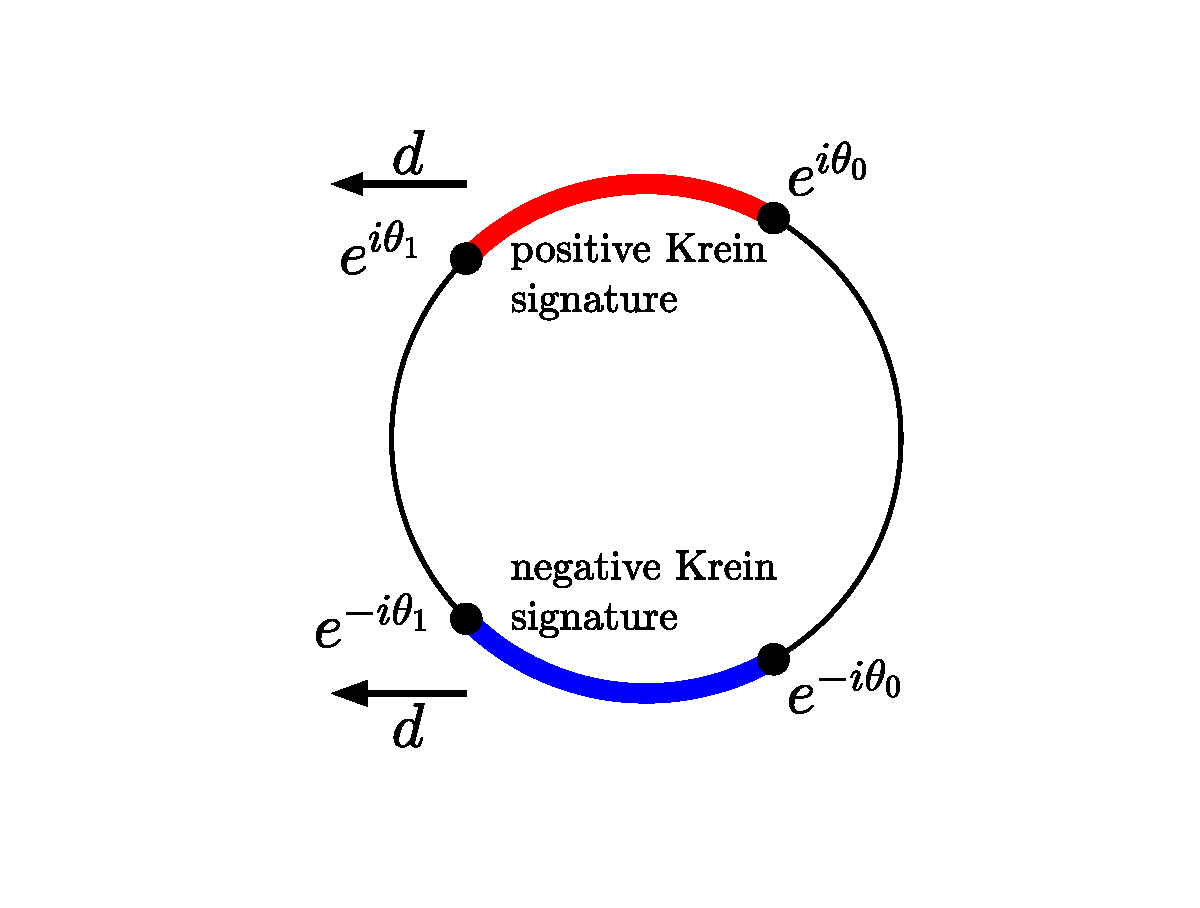
\includegraphics[width=7.5cm]{contspeccartoon1.eps} &
	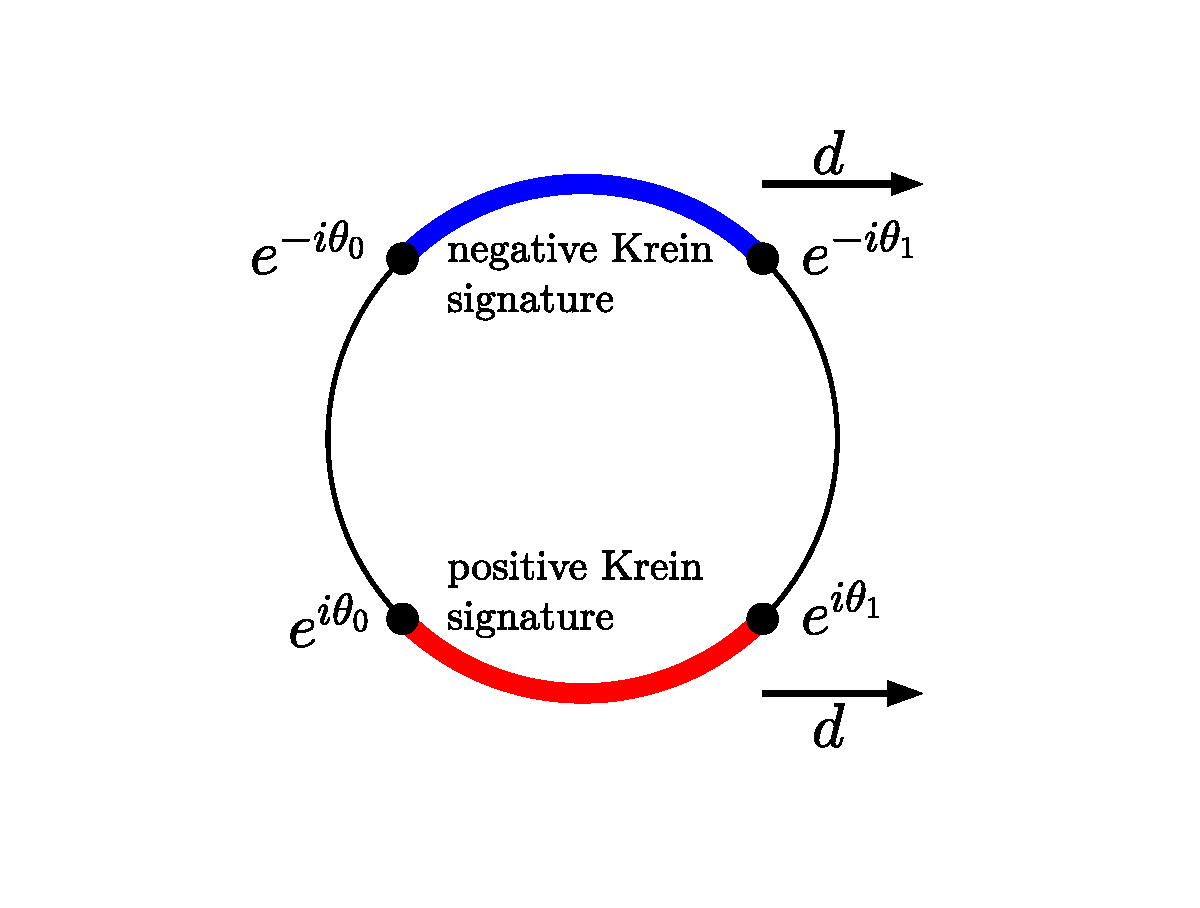
\includegraphics[width=7.5cm]{contspeccartoon2.eps}
	\end{tabular}
	\end{center}
	\caption{Cartoon showing continuous spectrum bands on the unit circle for $T \in (n \pi, (n+1)\pi)$ with $n$ even (left) and $n$ odd (right). Krein signature of bands is indicated, and bands grow in the direction of the arrow with increasing $d$.}
	\label{fig:bands}
\end{figure}

\subsection{Spatial dynamics}

We now reformulate both the DKG equation \cref{eq:DKG} and the eigenvalue problem \cref{eq:DKGeig} using a spatial dynamics approach, as in \cites{Parker2020,Parker2021}. Let $\uvec(t)$ be a breather solution to \cref{eq:DKG}, and define $U(n)$ by $U(n) = (u(n), \tilde{u}(n)) = ( u_n, u_{n-1} )$. Then equation \cref{eq:DKG} is equivalent to the lattice dynamical system
\begin{equation}\label{eq:dynEq}
U(n+1) = F(U(n)),
\end{equation}
where
\begin{equation}\label{eq:F}
F\begin{pmatrix}u \\ \tilde{u} \end{pmatrix} = 
\begin{pmatrix}2u  + \dfrac{1}{d}f(u) + \dfrac{1}{d} \partial_t^2 u - \tilde{u} \\
u
\end{pmatrix}.
\end{equation}
We note that since $f$ is a odd function, if $U(n)$ is a solution to \cref{eq:dynEq}, then $-U(n)$ is as well. The eigenvalue problem \cref{eq:DKGeig} can similarly be written as 
\begin{equation}\label{eq:dynEVP}
W(n+1) = \left[ DF(U(n)) + (2 \lambda \partial_t + \lambda^2) B \right] W(n),
\end{equation}
where
\begin{equation}\label{eq:DFU}
DF(U(n)) = \begin{pmatrix}
2 + \dfrac{f'(u(n))}{d} + \dfrac{1}{d}\partial_t^2  & -1 \\ 1 & 0
\end{pmatrix}, \qquad
B = \begin{pmatrix} 1 & 0 \\ 0 & 0 \end{pmatrix}.
\end{equation}
The zero function $U(n) = 0$ is an equilibrium solution to \cref{eq:dynEq}. The standard procedure (see, for example, \cites{Parker2021,Parker2020,Sandstede1998}) is to consider $U(n)$ to be a homoclinic orbit of the equilibrium at 0. The complication here is that for the difference equation \cref{eq:dynEq} to be well-posed, we require $U(n) \in C_\per^\infty([0,T],\R^2)$ for all $n$, rather than just $H^2_\per([0,T], \R^2)$, since each application of \cref{eq:dynEq} involves differentiating twice with respect to $t$. Since $C_\per^\infty([0,T])$ is not a closed subspace of $L^2([0,T])$, it is not straightforward to adapt the stable manifold theorem and results on exponential dichotomies to this problem, even if $DF(0)$ has the desired spectral properties. As an alternative, we will consider a finite-dimensional approximation, where we project the problem onto a finite-dimensional subspace of $L_\per^2([0,T])$. Roughly, this subspace consists of the first $N$ Fourier modes of the standard basis for $L_\per^2([0,T])$. Although this is a limited result, we note that since $U(n)$ is smooth, its Fourier coefficients decay exponentially. Since we can take $N$ as large as we like, this is a very good approximation. In addition, since the numerical simulations are performed using Fourier spectral methods, this theory applies directly to the numerical discretization. Before we formulate our approximation, we prove some important results about the spectrum of $DF(0)$.

\subsection{Spectrum of \texorpdfstring{$DF(0)$}{DF(0)}}

The linearization of \cref{eq:dynEq} about the equilibrium at 0 is the constant coefficient linear operator 
\begin{equation}\label{eq:DF0}
DF(0) = \begin{pmatrix}
\dfrac{1}{d}\partial_t^2 + \dfrac{f'(0)}{d} + 2 & -1 \\ 1 & 0
\end{pmatrix},
\end{equation}
which is invertible with inverse
\begin{equation}\label{eq:DF0inv}
DF(0)^{-1} = \begin{pmatrix}
0 & 1 \\ -1 & \dfrac{1}{d}\partial_t^2 + \dfrac{f'(0)}{d} + 2
\end{pmatrix}
\end{equation}
First, we determine the eigenvalues and eigenfunctions of $DF(0)$.

\begin{lemma}\label{lemma:DF0eigs}
The set of eigenvalues of $DF(0)$ is given by $\bigcup_{k \in \Z} \{\lambda_k, \lambda_k^{-1} \}$, where 
\begin{equation}\label{eq:DF0lambdak}
\lambda_k = \frac{1}{2}\left( r_k + \sqrt{r_k^2 - 4} \right), \quad r_k = -\frac{4 k^2 \pi^2}{d T^2} + \frac{f'(0)}{d} + 2.
\end{equation}
For $k \neq 0$, these have algebraic multiplicity 2, since $\lambda_{-k} = \lambda_k$. For each $k \in \Z$, $\{\lambda_k, \lambda_k^{-1} \}$ is either real, or a complex conjugate pair on the unit circle. The eigenfunctions corresponding to $\left\{ \lambda_k, \lambda_k^{-1} \right\}$ are $\left\{ U_k(t), U_k^{-1}(t) \right\}$, which are defined, up to constant multiple, by 
\begin{equation}\label{eq:DF0eigenfns}
\begin{aligned}
U_k(t) &= \begin{pmatrix}v_k(t) \\ \lambda_k^{-1}  v_k(t) \end{pmatrix}, \quad
U_k^{-1}(t) = \begin{pmatrix}v_k(t) \\ \lambda_k v_k(t) \end{pmatrix}, \quad
v_k(t) = \frac{1}{T} \exp\left( i \frac{2 \pi k t}{T} \right).
\end{aligned}
\end{equation}
\end{lemma}
\begin{proof}
Consider the eigenvalue problem $DF(0) U(t) = \lambda U(t)$ on $H^2_\per([0,T],\R^2)$, where $U(t) = (v(t), w(t))^T$. We note that $\lambda = 0$ is not an eigenvalue, since that implies $v = w = 0$. The eigenvalue problem then reduces to the system of equations
\begin{align}\label{eq:DF0EVPsystem}
\left( \frac{1}{d}\partial_t^2 + \frac{f'(0)}{d} + 2 \right) v(t) = \left( \lambda + \frac{1}{\lambda} \right) v(t), \quad
w = \frac{1}{\lambda} v(t).
\end{align}
Letting $r = \lambda + \frac{1}{\lambda}$ and using the periodic boundary conditions $v(T) = v(0)$, the set of solutions to \cref{eq:DF0EVPsystem} is given by
\begin{align}
v_k(t) &= \frac{1}{T} \exp\left( i \frac{2 \pi k t}{T} \right), \quad r_k = -\frac{4 k^2 \pi^2}{d T^2} + \frac{f'(0)}{d} + 2 && k \in \Z,
\end{align}
where the functions $v_k(t)$ have been normalized. The corresponding eigenvalues of $DF(0)$ are then given by $\left\{ \lambda_k, \lambda_k^{-1} \right\}$, where $\lambda_k$ is defined by \cref{eq:DF0lambdak}, and the corresponding eigenfunctions are given by \cref{eq:DF0eigenfns}. The pair $\left\{ \lambda_k, \lambda_k^{-1} \right\}$ is real if $|r_k| \geq 2$, and is complex with modulus 1 if $|r_k| < 2$.
\end{proof}

We note that the spectrum of $DF(0)$ depends on both the coupling parameter $d$ and the period $T$. It follows from \cref{lemma:DF0eigs} that the spectrum of $DF(0)$ is bounded away from the unit circle provided $|r_k| > 2$ for all $k$. The following lemma gives some conditions on $T$ and $d$ to guarantee that this is the case.

\begin{lemma}\label{lemma:DF0hyp}
The spectrum of $DF(0)$ is bounded away from the unit circle if, for a specific nonnegative integer $k$, $T$ and $d$ are chosen so that
\begin{equation}\label{eq:Tdpair}
\frac{2 k \pi}{\sqrt{f'(0)}} < T < \frac{2 (k+1) \pi}{\sqrt{f'(0)}} , \qquad 0 < d < \frac{(k+1)^2\pi^2}{T^2} - \frac{f'(0)}{4}.
\end{equation}
\begin{proof}
Since $f'(0) > 0$, $r_0 = 2 + \frac{1}{d}f'(0) > 2$, and $r_k$ is strictly decreasing in $k$, with $r_k \rightarrow -\infty$ as $k \rightarrow \infty$. Thus $|r_k| > 2$ for all $k$ if $r_k > 2$ and $r_{k+1} < -2$ for some nonnegative integer $k$, from which the conditions \cref{eq:Tdpair} follow.
\end{proof}
\end{lemma}

We take the following assumption on the spectrum of $DF(0)$, which is the analogue to hyperbolicity in the finite-dimensional case.

\begin{hypothesis}\label{hyp:hyp}
The coupling constant $d$ and period $T$ are chosen so that the spectrum of $DF(0)$ is bounded away from the unit circle.
\end{hypothesis}

% Finally, we show that the eigenfunctions of $DF(0)$ are a Hilbert basis for $L^2_\per([0,T],\R^2)$.
% \begin{lemma}\label{lemma:DF0basis}
% Assume \cref{hyp:hyp}. The set of eigenfunctions $\bigcup_{k \in \Z} \{U_k(t) , U_k^{-1}(t) \}$ of $DF(0)$ is a Hilbert basis for $L^2_\per([0,T],\R^2)$, i.e. every function $Y(t) \in L^2_\per([0,T],\R^2)$ can be written uniquely as
% \begin{equation}\label{eq:yinDF0basis}
% Y(t) = \sum_{k \in \Z} a_k U_k(t) + \sum_{k \in \Z} b_k U^{-1}_k(t),
% \end{equation}
% where $a_k, b_k \in \C$ and the sum converges for all $Y(t)$.
% \begin{proof}
% Letting $v_k(t) = \frac{1}{T} \exp\left( i \frac{2 \pi k t}{T} \right)$, the set $\{ v_k(t) : k \in \Z \}$ is an orthonormal basis for $L^2_\per([0,T],\R)$. It follows that the set $\bigcup_{k \in \Z} \{Z^1_k(t) , Z^2_k(t) \}$ is an orthonormal basis for $L^2_\per([0,T],\R^2)$, where $Z^1_k(t) = (v_k(t), 0)^T$ and $Z^2_k(t) = (0, v_k(t))^T$. Therefore, there exist unique scalars $c_k, d_k \in \C$ such that
% \begin{equation*}
% Y(t) = \sum_{k \in \Z} c_k Z^1_k(t) + \sum_{k \in \Z} d_k Z^2_k(t),
% \end{equation*}
% and the sum converges for all $Y(t)$. Equation \cref{eq:yinDF0basis} follows by taking
% \[
% a_k = \frac{1}{\lambda_k^2 - 1}\left(-c_k + \lambda_k d_k \right), \quad
% b_k = \frac{1}{\lambda_k^2 - 1}\left( \lambda_k^2 c_k - \lambda_k d_k \right),
% \]
% where $\lambda_k$ is defined in \cref{eq:DF0lambdak}, and $\lambda_k^2 \neq 1$ by \cref{hyp:hyp}.
% \end{proof}
% \end{lemma}

\subsection{Finite dimensional approximation}

We now define our finite dimensional approximation for \cref{eq:dynEq}. For $M \geq 1$, let 
\begin{equation}\label{eq:XM}
X_M = \spn\left\{ \bigcup_{k = -M}^M v_k(t) \right\}, \qquad
v_k(t) = \frac{1}{T} \exp\left( i \frac{2 \pi k t}{T} \right).
\end{equation}
be the $(2M+1)$-dimensional subspace of $L_\per^2([0,T])$ spanned by the Fourier basis functions with wavenumber $|k| \leq M$, and let $P_M: L_\per^2([0,T]) \rightarrow X_M$, defined by
\begin{equation}\label{eq:PM}
P_M u(t) = \sum_{k=-M}^M \langle u, v_k \rangle_{L^2([0,T])} v_k(t)
= \sum_{k=-M}^M \left( \int_0^T u(s) \overline{v_k(s)} ds \right) v_k(t)
\end{equation}
be the corresponding projection operator, which is smooth in $t$ as long as $u$ is also smooth in $t$. Let $X_{M,e}$ be the $(M+1)$-dimensional subspace of $X_M$ comprising functions which are even in $t$, i.e.
\begin{equation}
X_{M,e} = \left\{ f \in X_M : f(-t) = f(t) \text{ for all }t \in \R \right\}.
\end{equation}
% An orthonormal basis for $X_{M,e}$ is $\left\{ \tilde{v}_k(t) \right\}_{k=0}^M$, where
% \begin{equation}\label{eq:vktilde}
% \tilde{v}_k(t) = \begin{cases}
% \frac{1}{T} & k = 0 \\
% \frac{2}{T} \cos\left( \frac{2 \pi k t}{T} \right) & k = 1, \dots, M.
% \end{cases}
% \end{equation}
Applying the projection $P_M$ to both components of \cref{eq:dynEq}, i.e. projecting onto $X_M^2$, we obtain
\begin{equation}
\begin{pmatrix}P_M u(n+1) \\ P_M \tilde{u}(n+1) \end{pmatrix} = 
\begin{pmatrix}2 P_M u  + \dfrac{1}{d}P_M f(u) + \dfrac{1}{d} P_M \partial_t^2 u - P_M \tilde{u} \\
P_M u
\end{pmatrix}.
\end{equation}
% The operators $P_M$ and $\partial_t$ commute, since 
% \begin{align*}
% \langle \dot{u}, v_k \rangle v_k &= -\langle u, \dot{v}_k \rangle v_k
% = -\left\langle u, \frac{2 \pi i k}{T} v_k \right\rangle v_k \\
% &= -\left( -\frac{2 \pi i k}{T} \right) \langle u, v_k \rangle v_k
% = \langle u, v_k \rangle \left( \frac{2 \pi i k}{T} \right) v_k 
% = \langle u, v_k \rangle \dot{v}_k,
% \end{align*}
% where we used the fact that the differentiation operator is anti-self-adjoint, and the inner product is conjugate linear in the second component. It follows that $P_M$ and $\partial_t^2$ commute. 
While the projection $P_M$ commutes with the differentiation operator $\partial_t^2$, in general it not the case that $P_M f(u) = f(P_M u)$. However, since $u$ is smooth, $(I-P_M)u$ will be small for sufficiently large $M$, thus we expand $f(u)$ as
\[
f(u) = f( P_M u + (I-P_M)u) = f(P_M u) + \mathcal{O}((I-P_M)u)
\]
and keep only the first term to get the approximate system on $X_M^2$
\begin{align}\label{eq:dynEqM}
U(n+1) &= F_M(U(n)) && U(n) \in X_M^2,
\end{align}
where
\begin{equation}\label{eq:FM}
F_M\begin{pmatrix}u \\ \tilde{u} \end{pmatrix} = 
\begin{pmatrix}2u  + \dfrac{1}{d}g(u) + \dfrac{1}{d} \partial_t^2 u - \tilde{u} \\
u
\end{pmatrix}
\end{equation}
and $g: X_M \rightarrow X_M$ is defined by $g = P_M f$. When $u = 0$, $g(0) = P_M f(0) = 0$, and $g'(0) = P_M f'(0) = f'(0)$, since $f'(0)$ is a constant function, which is in $X_M$ for all $M$. Furthermore, since $f$ is an odd function, so is $g$, thus $F_M(-U) = -F_M(U)$. It follows that if $U(n)$ is a solution to \cref{eq:dynEqM}, so is $-U(n)$. If $U(n) = (u(n), \tilde{u}(n))^T$ is a solution to \cref{eq:dynEqM}, then, by taking $u_n = u(n)$, the first component $u(n)$ is a breather solution to the approximate DKG equation
\begin{equation}\label{eq:DKGapprox}
\begin{aligned}
\ddot{u}_n &= d (\Delta_2 u)_n - g(u_n) && u_n \in X_M.
\end{aligned}
\end{equation}
Linearization of \cref{eq:DKGapprox} about a solution $\uvec \in \ell^2(\Z, X_M)$ yields the eigenvalue problem
\begin{equation}\label{eq:DKGMeigL}
\begin{aligned}
d (\Delta_2 w)_n - g'(u_n)w_n - \ddot{w}_n = 2 \lambda \dot{w}_n + \lambda^2 w_n,
\end{aligned}
\end{equation}
which we write as $\calL_M(\uvec)\wvec = (2 \lambda \partial_t + \lambda^2 )\wvec$, where 
$\calL_M(\uvec)$ is the linear operator on $\ell^2(\Z, X_M)$ defined by the LHS of \cref{eq:DKGMeigL}.
As i 

\begin{equation}\label{eq:dynEVP}
W(n+1) = \left[ DF(U(n)) + (2 \lambda \partial_t + \lambda^2) B \right] W(n),
\end{equation}
where
\begin{equation}\label{eq:DFU}
DF(U(n)) = \begin{pmatrix}
2 + \dfrac{f'(u(n))}{d} + \dfrac{1}{d}\partial_t^2  & -1 \\ 1 & 0
\end{pmatrix}, \qquad
B = \begin{pmatrix} 1 & 0 \\ 0 & 0 \end{pmatrix}.
\end{equation}




Let $\{\tau(s) : s \in \R\}$ be the one-parameter group of unitary translation operators on $X_M^2$, defined by $[\tau(s)]U(\cdot) = U(\cdot - s)$, which has infinitesimal generator $\tau'(0) = \partial_t$. We note that this group is well-defined on $X_M^2$, since 
\[
\tau(s) v_k(t) 
\frac{1}{T} \exp\left( i \frac{2 \pi k (t-s)}{T}\right) 
= \exp\left( -i \frac{2 \pi k s}{T} \right) \frac{1}{T} \exp\left( i \frac{2 \pi k t}{T}\right) 
= \exp\left( -i \frac{2 \pi k s}{T} \right) v_k(t),
\]
i.e. the group action multiplies a basis element by a constant. In fact, the eigenvalue at 0 of \cref{eq:DKGeig} is a result of this translational symmetry. The function $F_M$ from \cref{eq:dynEqM} (as well as $F$ from the full system \cref{eq:dynEq}) commutes with this one-parameter group, i.e. $F(\tau(s) U) = \tau(s) F(U)$. It is cruicial to note that this symmetry is lost if we consider the problem \cref{eq:dynEqM} on $X_{M,e}^2$, since the space of even functions is not translation invariant. 

\section{Multi-breathers}

Our strategy will be to first prove that multi-breathers exist on the subspace $X_{M,e}^2$ of even functions. Since there is no translational symmetry, the stable and unstable manifolds of the origin will intersect transversely, which greatly simplifies the analysis. This parallels the restriction in \cite{Pelinovsky2012} to breathers which are even in $t$, and is consistent with the odd symmetry of the nonlinearity $f$. 
Once that is accomplished, we will return to the full space $X_{M}^2$ for the eigenvalue problem, and use Lin's method as in \cites{Parker2021,Parker2020,Sandstede1998} to construct the interaction eigenfunctions as piecewise linear combinations of the eigenfunction corresponding to translation symmetry. This technique is similar to the one we employed in \cite{Parker2020} for DNLS, where, to prove the existence of multi-pulses, we removed the gauge symmetry by restricting the problem to real-valued solutions.

\subsection{Primary breather}

To accomplish this, we will take the existence of a primary, single-site breather as a hypothesis. 
Fix $d$ and $T$ such that \cref{hyp:hyp} holds. First, we consider the approximate system \cref{eq:dynEqM} on $X_{M,e}^2$.  Since $g'(0) = f'(0)$, the linear operator $DF_M(0)$ on $X_{M,e}^2$ is also given by \cref{eq:DF0}. By \cref{lemma:DF0eigs}, the $2M+2$ eigenvalues of $DF_M(0)$ on $X_{M,e}^2$ are given by $S_M = \bigcup_{k=0}^M \{\lambda_k, \lambda_k^{-1} \}$, where these are defined in the statement of \cref{lemma:DF0eigs}. By our choice of $d$ and $T$ in \cref{hyp:hyp}, the spectrum of $DF_M(0)$ is real and does not intersect the unit circle, thus 0 is a hyperbolic equilibrium point of \cref{eq:dynEqM}. Define the stable and unstable subsets of the spectrum of $DF_M(0)$ by
\[
S_M^s = \{ \lambda \in S_M : |\lambda| < 1\}, \qquad S_M^u = \{ \lambda \in S_M : |\lambda| > 1\}.
\]
By symmetry, $|S_M^s| = |S_M^u| = M+1$. Define
\begin{equation}\label{eq:defrM}
r_M = \min \{ |\lambda| : \lambda \in S_M^u, |\lambda| > 1 \}.
\end{equation}
Since $X_{M,e}^2$ is finite-dimensional, the stable manifold holds. For each $M \geq 1$, let $W_{M,e}^s(0)$ and $W_{M,e}^u(0)$ be the $(M+1)$-dimensional stable and unstable manifolds, which are subsets of $X_{M,e}^2$. A breather solution to \cref{eq:dynEqM} is a homoclinic orbit to the equilibrium point at 0 which lies in the intersection of the stable and unstable manifolds. We take the existence of such a solution as a hypothesis.

\begin{hypothesis}\label{hyp:breather}
Let $d$ and $T$ be chosen according to \cref{hyp:hyp}. There exists a positive integer $M_0$ such that for all $M \geq M_0$, the stable and unstable manifolds $W_{M,e}^s(0)$ and $W_{M,e}^u(0)$ intersect transversely in $X_{M,e}^2$ in a homoclinic orbit $Q_M(n) = (q_M(n), \tilde{q}_M(n))^T$. 
\end{hypothesis}

In addition, we obtain the estimate 
\begin{equation}\label{eq:U1decayest}
\|Q_M(n)\|_{X_M} \leq C r_M^{-|n|}
\end{equation}
as a consequence of the stable manifold theorem.

We now consider \cref{eq:dynEqM} on $X_M^2$. The spectrum of $DF(0)$ on $X_M^2$ is exactly the same as that on $X_{M,e}^2$, except the eigenvalues corresponding to $k = 1, \dots, M$ have multiplicity of 2. It follows that 0 is also a hyperbolic equilibrium of \cref{eq:dynEqM} on $X_M^2$. Let $W_M^s(0)$ and $W_M^u(0)$ be the $(2M+1)$-dimensional stable and unstable manifolds, which are subsets of $X_M^2$. For $M \geq M_0$, $Q_M(n)$ is also a homoclinic orbit connecting these stable and unstable manifolds. In the next hypothesis, we assume that this intersection is non-degenerate.

\begin{hypothesis}\label{hyp:breathernondegen}
Let $d$ and $T$ be chosen according to \cref{hyp:hyp}, and let $M_0$ and $Q_M(n)$ be as in \cref{hyp:breather}. Then for all $M \geq M_0$, the stable and unstable manifolds $W_M^s(0)$ and $W_M^u(0)$ have a one-dimensional intersection in $Q_M(n)$.
\end{hypothesis}

The variational equation is the linearization of \cref{eq:dynEqM} on $X_M^2$ about the homoclinic orbit solution $Q_M(n)$, given by
\begin{equation}\label{eq:vareq}
\begin{aligned}
W(n+1) &= DF_M(Q_M(n)) W(n) && W(n) \in X_M^2.
\end{aligned}
\end{equation}
Since the tangent spaces of $W_M^s(0)$ and $W_M^u(0)$ have a one-dimensional intersection by \cref{hyp:breathernondegen}, it follows that $\dot{Q}_M(n)$ is the unique, bounded solution to \cref{eq:vareq}, up to scalar multiples. ($\dot{Q}_M(n)$ is not a solution to \cref{eq:vareq} on $X_{M,e}^2$, since it is an odd function). We can thus decompose the tangent spaces to $W_M^u(0)$ and $W_M^s(0)$ at $U_M^1(0)$ as
\begin{equation}\label{eq:TWdecomp}
T_{Q_M(0)}W^u(0) = \R \dot{Q}_M(0) \oplus Y_M^-, \qquad  
T_{Q_M(0)}W^s(0) = \R \dot{Q}_M(0) \oplus Y_M^+,
\end{equation}
where $\dim Y_M^- = \dim Y_M^+ = 2M$. In addition, the adjoint variational equation
\begin{equation}\label{eq:adjvareq}
Z(n) = DF_M(Q_M(n))^* Z(n+1)
\end{equation}
has a unique bounded solution, given by
\begin{equation}\label{eq:Z1}
Z_M(n) = (-\dot{q}_M(n-1), \dot{q}_M(n))^T,
\end{equation}
and $Z_M(0) \perp \R \dot{Q}_M(0) \oplus Y_M^- \oplus Y_M^+$ by \cite{Parker2020}*{Lemma 1}. We can thus decompose $X_M^2$ as
\begin{equation}\label{eq:Xdecomp}
X_M^2= \R \dot{Q}_M(0) \oplus Y_M^- \oplus Y_M^+ \oplus \R Z_M(0).
\end{equation}

\subsection{Existence}

We construct a multi-breather on $X_{M,e}$ by splicing together multiple copies of the primary breather $Q_M(n)$ end-to-end as in \cites{Parker2020,Sandstede1998}. We characterize a multi-breather in the following way. Let $m > 1$ be the total number of copies of the primary breather in the chain. Let $N_i$ ($i = 1, \dots, m-1$) be the distances (in lattice points) between the center point of each breather. We seek to construct a solution $U(n)$ which can be written piecewise in the form
\begin{equation}\label{eq:Upiecewise}
\begin{aligned}
U_i^-(n) &= \sigma_i Q_M(n) + \tilde{U}_i^-(n) && n \in [-N_{i-1}^-, 0] && \quad i = 1, \dots, m\\
U_i^+(n) &= \sigma_i Q_M(n) + \tilde{U}_i^+(n) && n \in [0, N_i^+] && \quad i = 1, \dots, m,
\end{aligned}
\end{equation}
where $\sigma_i \in \{1, -1\}$ represents the orientation of each copy of the primary breather, $N_i^+ = \lfloor \frac{N_i}{2} \rfloor$, $N_i^- = N_i - N_i^+$, and $N_0^- = N_m^+ = \infty$. Adjacent copies of the primary breather are in-phase if $\sigma_i \sigma_{i+1} = 1$ or out-of-phase if $\sigma_i \sigma_{i+1} = -1$. (Again, as in \cite{Pelinovsky2012}, other phase relations are not considered here). The functions $\tilde{U}_i^\pm(n)$ in \cref{eq:Upiecewise} are remainder terms, which will be small. We also define the characteristic distance
\begin{equation}\label{defN}
N = \frac{1}{2} \min\{ N_i \},
\end{equation}
which will be used in the estimates of the remainder terms $\tilde{U}_i^\pm(n)$. The individual pieces $U_i^\pm(n)$ are joined together end-to-end as in \cites{Sandstede1998,Knobloch2000,Parker2020,Parker2021} to create the multi-breather $U(n)$, which can be written in piecewise form as
\begin{equation}
\begin{aligned}
U(n) &= \begin{cases}
U_i^-\left( n - \sum_{j=1}^{i-1}N_j \right) & \sum_{j=1}^{i-1}N_j - N_{i-1}^- + 1 \leq n \leq \sum_{j=1}^{i-1}N_j \\
U_i^+\left( n - \sum_{j=1}^{i-1}N_j \right) & \sum_{j=1}^{i-1}N_j + 1 \leq n \leq \sum_{j=1}^{i-1}N_j + N_i^+
\end{cases}
&& i = 1, \dots, m,
\end{aligned}
\end{equation}
where we define $\sum_{j=1}^0 N_j = 0$. We then have the following existence theorem concerning the existence of multi-breathers on $X_{M,e}$. 

\begin{theorem}\label{th:multibreathers}
Assume \cref{hyp:hyp} and \cref{hyp:breather}, and let $M \geq M_0$, where $M_0$ is defined in \cref{hyp:breather}. Then there exists a positive integer $N_0$ with the following property. For all $m > 1$ and distances $N_i \geq N_0$, there exists a unique solution $U(n)$ which comprises, to leading order, $m$ sequential copies of the primary breather, and can be written piecewise in the form \cref{eq:Upiecewise}. For the remainder terms $\tilde{U}_i^\pm(n)$, we have the estimates
\begin{equation}\label{eq:Uestimates}
\begin{aligned}
\| \tilde{U}_i^-(n)\|_{X_M} &\leq C r_M^{-N_{i-1}^-} r_M^{-(N_{i-1}^- + n)} && \qquad n = 2, \dots, m\\
\|\tilde{U}_i^+(n) \|_{X_M} &\leq C r_M^{-N_i^+} r_M^{-(N_i^+ - n)} && \qquad n = 1, \dots, m-1 \\
\| \tilde{U}_1^-(n)\|_{X_M} &\leq C r_M^{-2N} r_M^{n} \\
\|\tilde{U}_m^+(n) \|_{X_M} &\leq C r_M^{-2N} r_M^{-n} .
\end{aligned}
\end{equation}
\begin{proof}
The proof is an adaptation of the proofs of theorems 1 and 3 in \cite{Parker2020}, and is very similar to the proof of \cite[Theorem 1]{Parker2021}. Since the stable and unstable manifolds $W_{M,e}^s(0)$ and $W_{M,e}^u(0)$ intersect transversely in $X_{M,e}$, the implementation of Lin's method does not involve jump conditions.
\end{proof}
\end{theorem}

\subsection{Spectral stability}



\begin{theorem}\label{th:spectrum}
Assume \cref{hyp:hyp}, \cref{hyp:breather}, and \cref{hyp:breathernondegen}. Let $U(n)$ be an $m$-component multi-breather constructed as in \cref{th:multibreathers} with distances $N_i$ and orientation parameters $\sigma_i$. Then there exists $\delta > 0$ small with the following property. $\lambda$ is an eigenvalue of the linearization about $\phi^m_n(t)$ if and only if $E(\lambda) = 0$, where
\begin{equation}\label{Elambda}
E(\lambda) = \det\left(A - \frac{1}{d}M \lambda^2 I + R(\lambda)\right).
\end{equation}
$A$ is the tridiagonal $m \times m$ matrix
\begin{align}\label{matrixA}
A &= \begin{pmatrix}
-a_1 & a_1 & & & \\
a_1 & -a_1 - a_2 & a_2 \\
& a_2 & -a_2 - a_3 & a_3 \\
& \ddots & & \ddots \\
& & & a_{m-1} & -a_{m-1}  \\
\end{pmatrix},
\end{align}
where
\begin{align*}
M &= \sum_{n = -\infty}^\infty \int_0^T \left( \dot{\phi}_n(t)^2 - 2 z_n(t) \ddot{\phi}_n(t)^2 \right) dt
\end{align*}
\begin{align*}
a_i &= \begin{cases}
\sigma_i \sigma_{i+1} \int_0^T \dot{\phi}_{\frac{N_i}{2}}(t)\left( \dot{\phi}_{\frac{N_i}{2}+1}(t) - \dot{\phi}_{\frac{N_i}{2}-1}(t) \right) dt & N_i \text{ even} \\
\sigma_i \sigma_{i+1} \int_0^T \left( \dot{\phi}_{\frac{N_i-1}{2}}(t)\dot{\phi}_{\frac{N_i+3}{2}}(t) - \dot{\phi}_{\frac{N_i+1}{2}}(t)\dot{\phi}_{\frac{N_i-3}{2}}(t) \right) dt & N_i \text{ odd}
\end{cases} \\
\end{align*}
and $z_n(t)$ is defined in \cref{eq:Lphikernel}. The remainder term has $R(\lambda)$ has some suitable bound.
\end{theorem}

\section{Numerical results}

\begin{figure}
	\begin{center}
	\begin{tabular}{cc}
	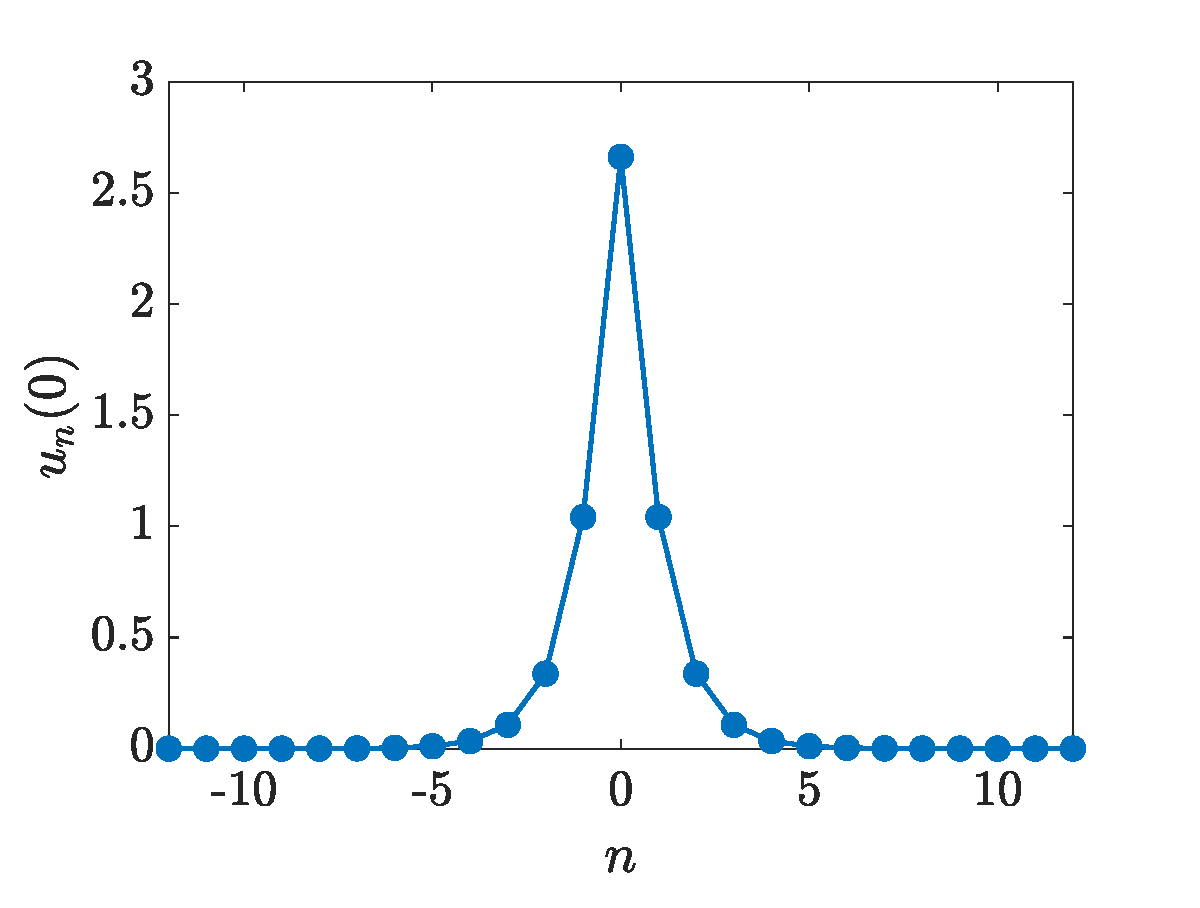
\includegraphics[width=7.5cm]{singleun0.eps} &
	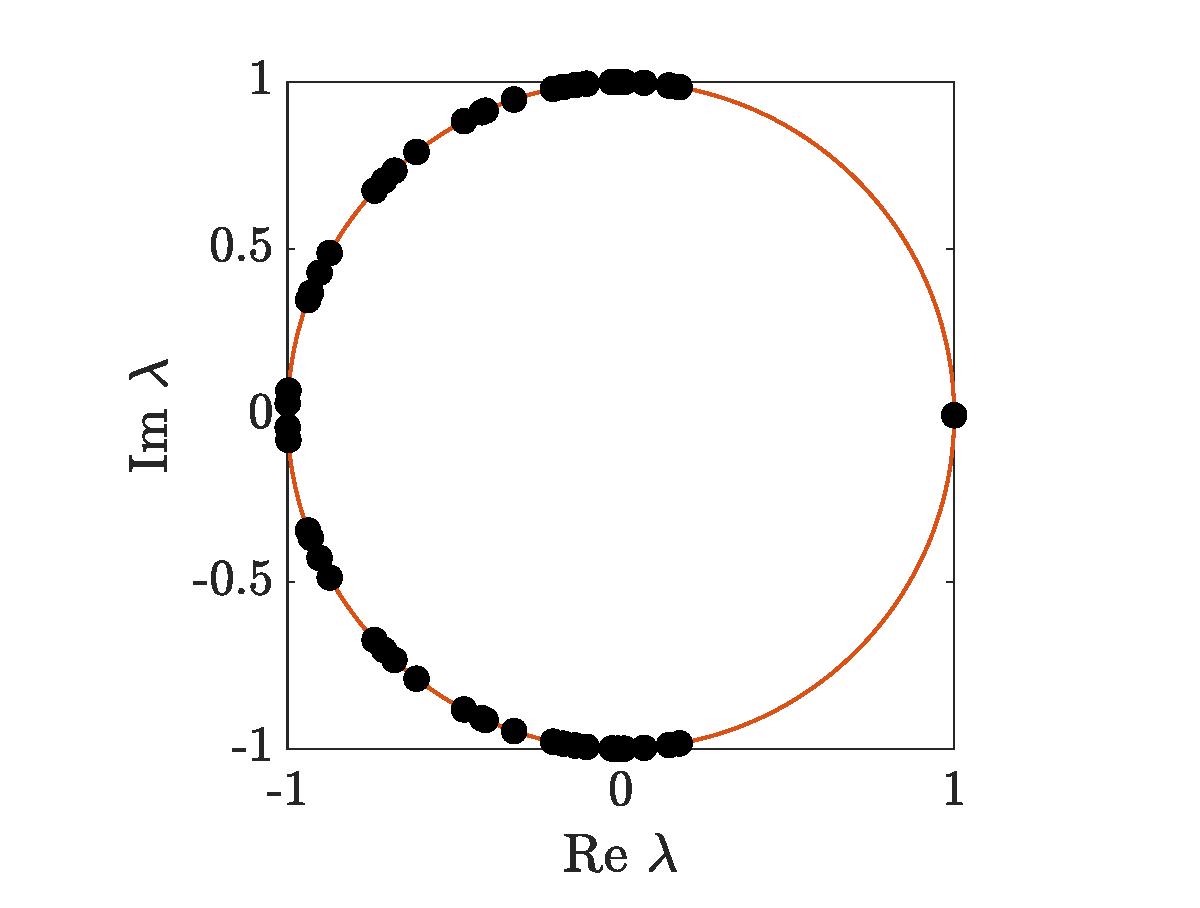
\includegraphics[width=7.5cm]{singlespec.eps} \\ 
	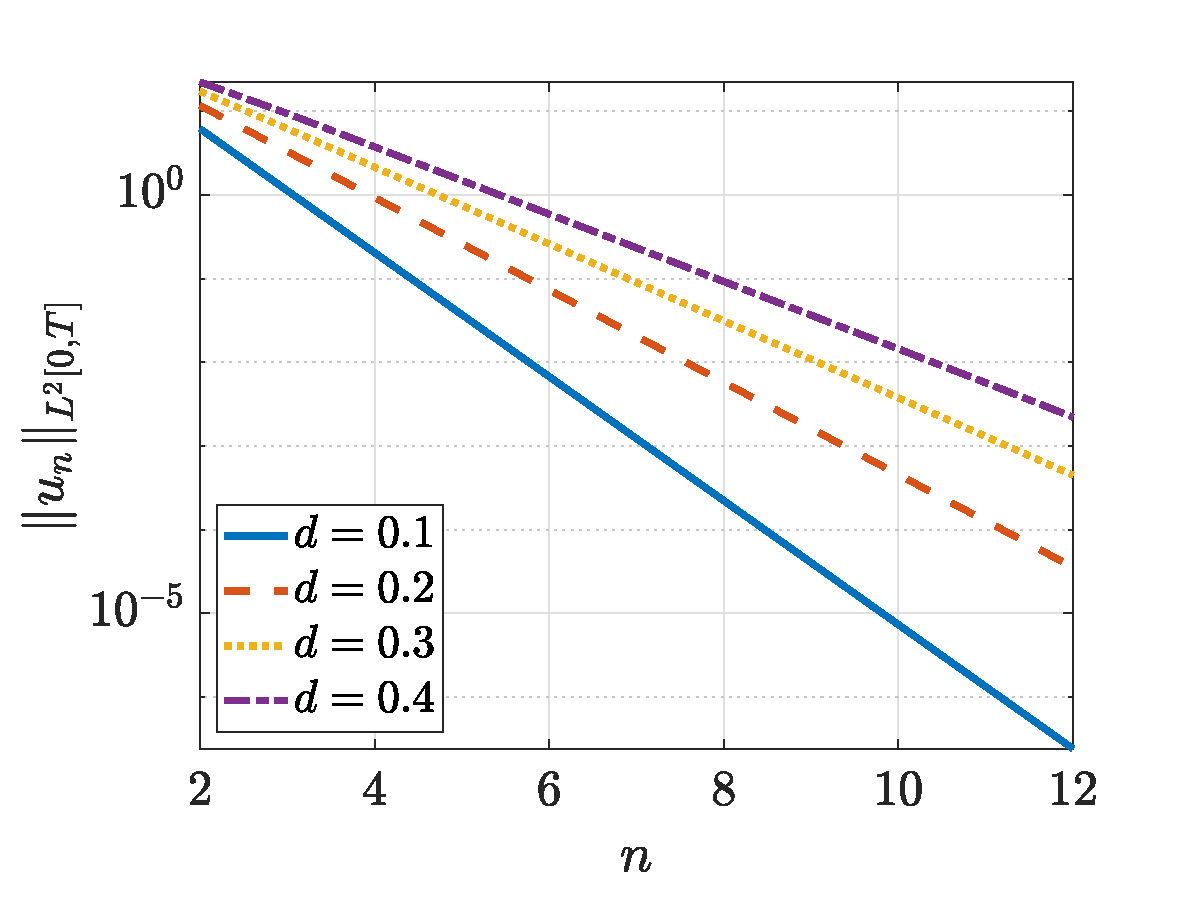
\includegraphics[width=7.5cm]{singledecay.eps} &
	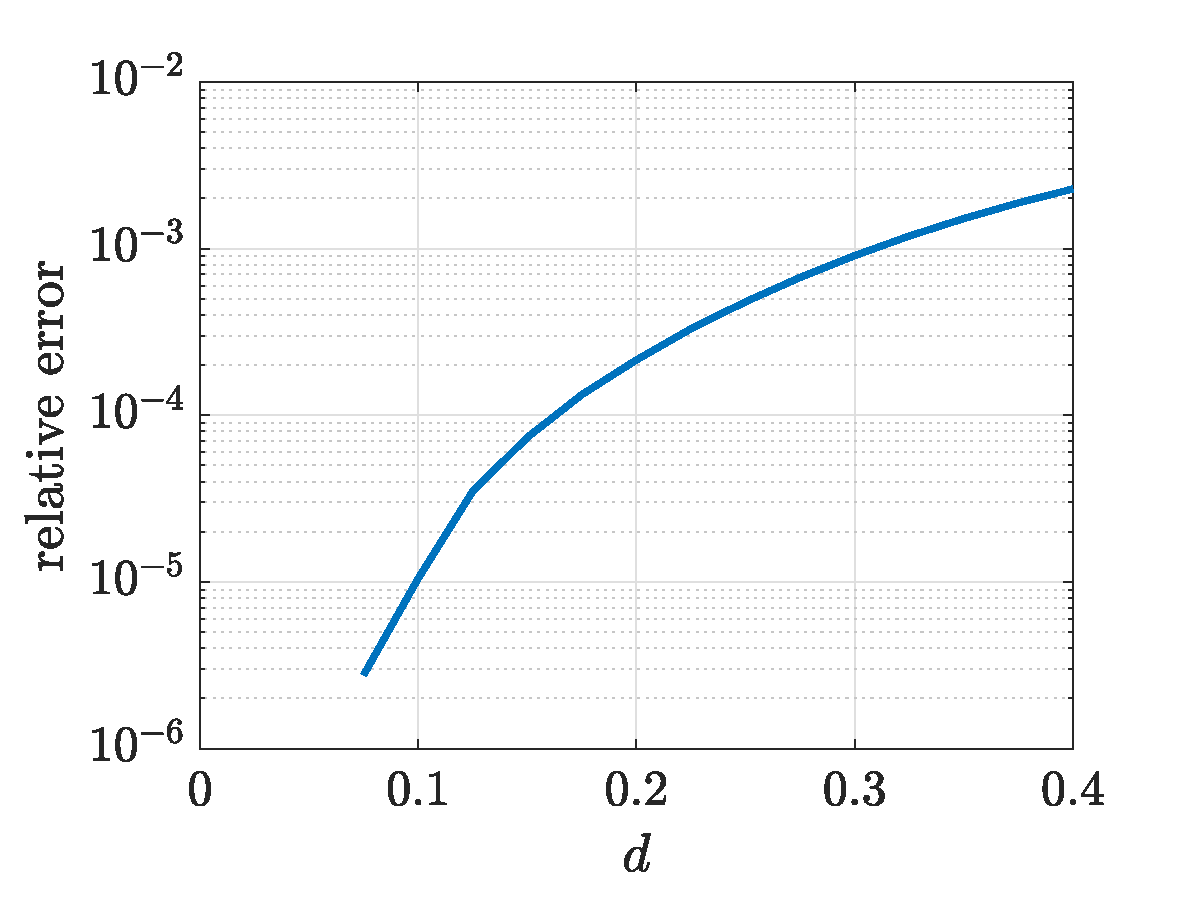
\includegraphics[width=7.5cm]{singledecayerror.eps}
	\end{tabular}
	\end{center}
	\caption{Single}
	\label{fig:single}
\end{figure}

\begin{figure}
	\begin{center}
	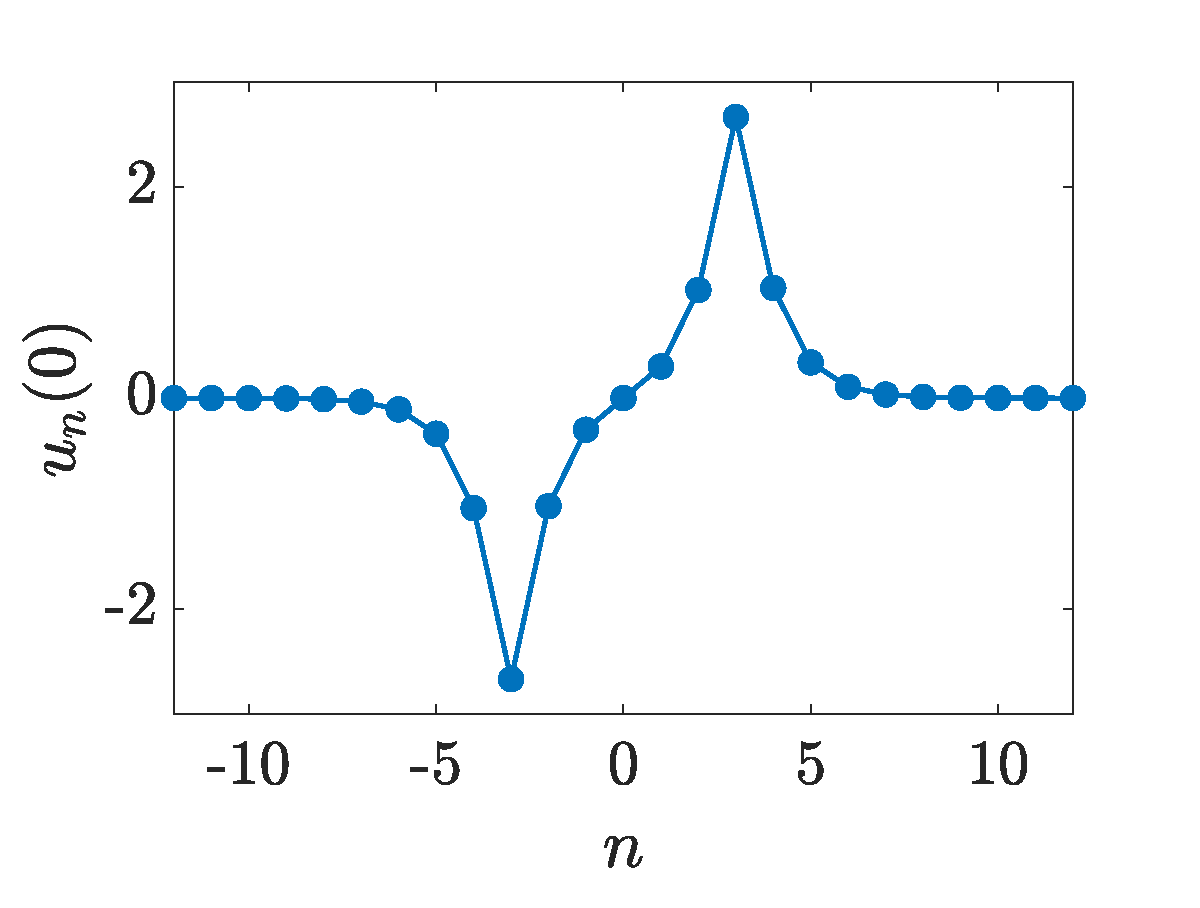
\includegraphics[width=5.5cm]{doubleun0.eps} \hspace{-0.5cm}
	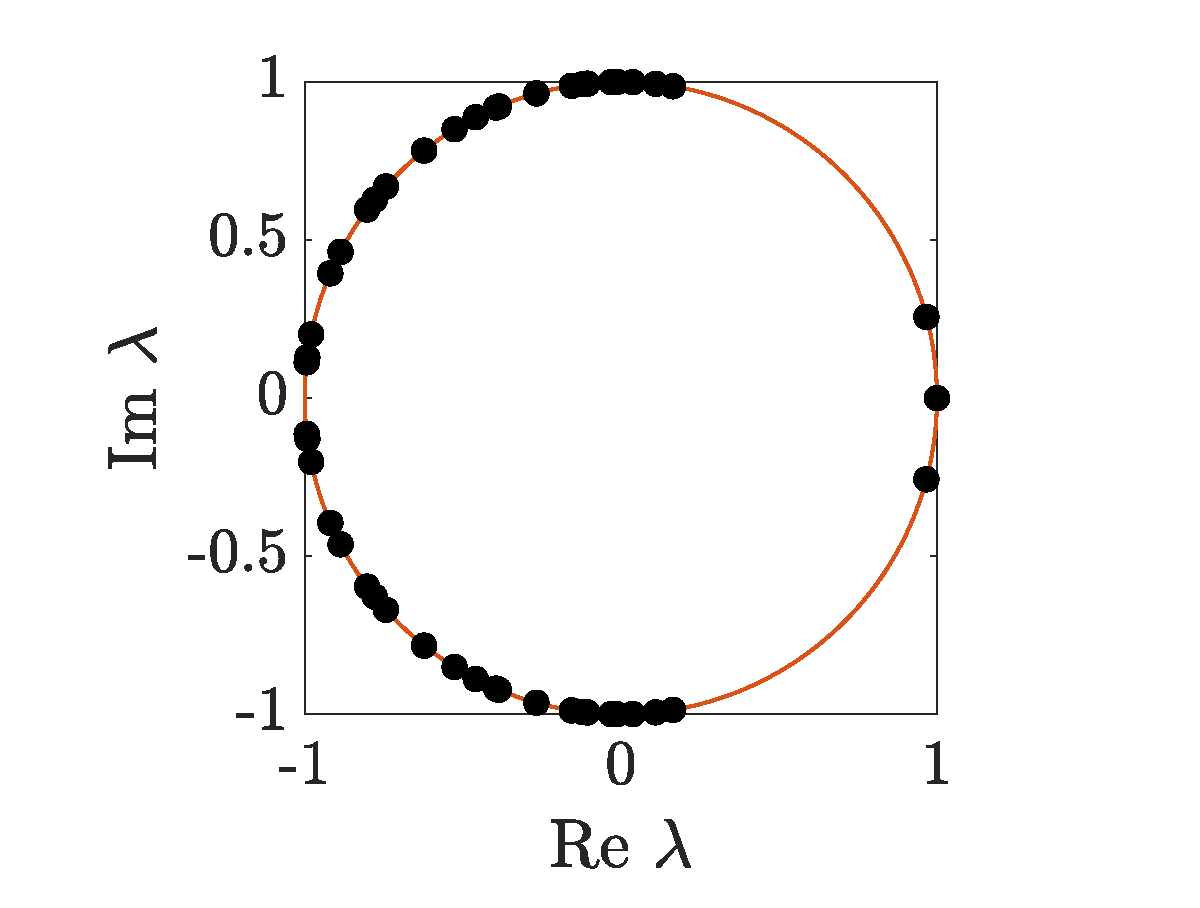
\includegraphics[width=5.5cm]{doublespec.eps} \hspace{-0.5cm}
	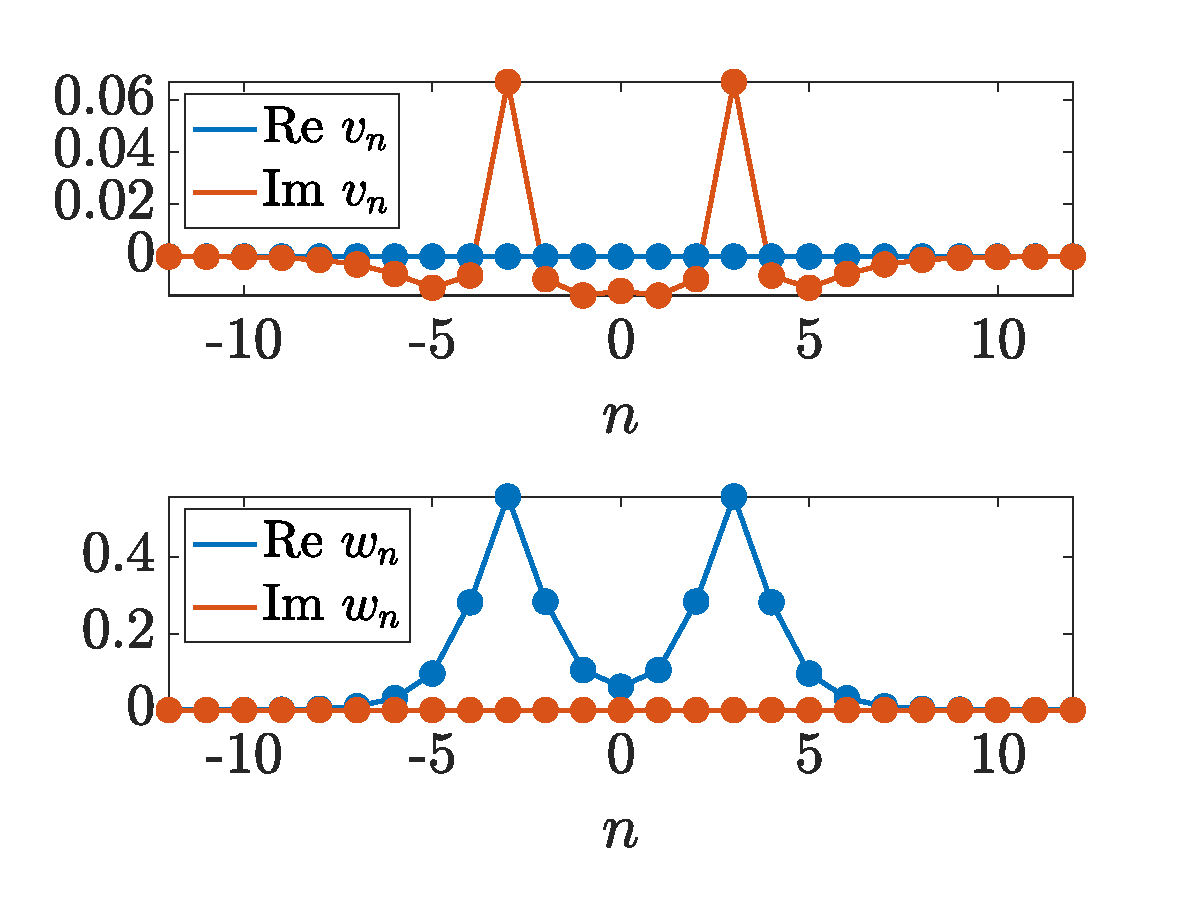
\includegraphics[width=5.5cm]{doubleinteig.eps} 
	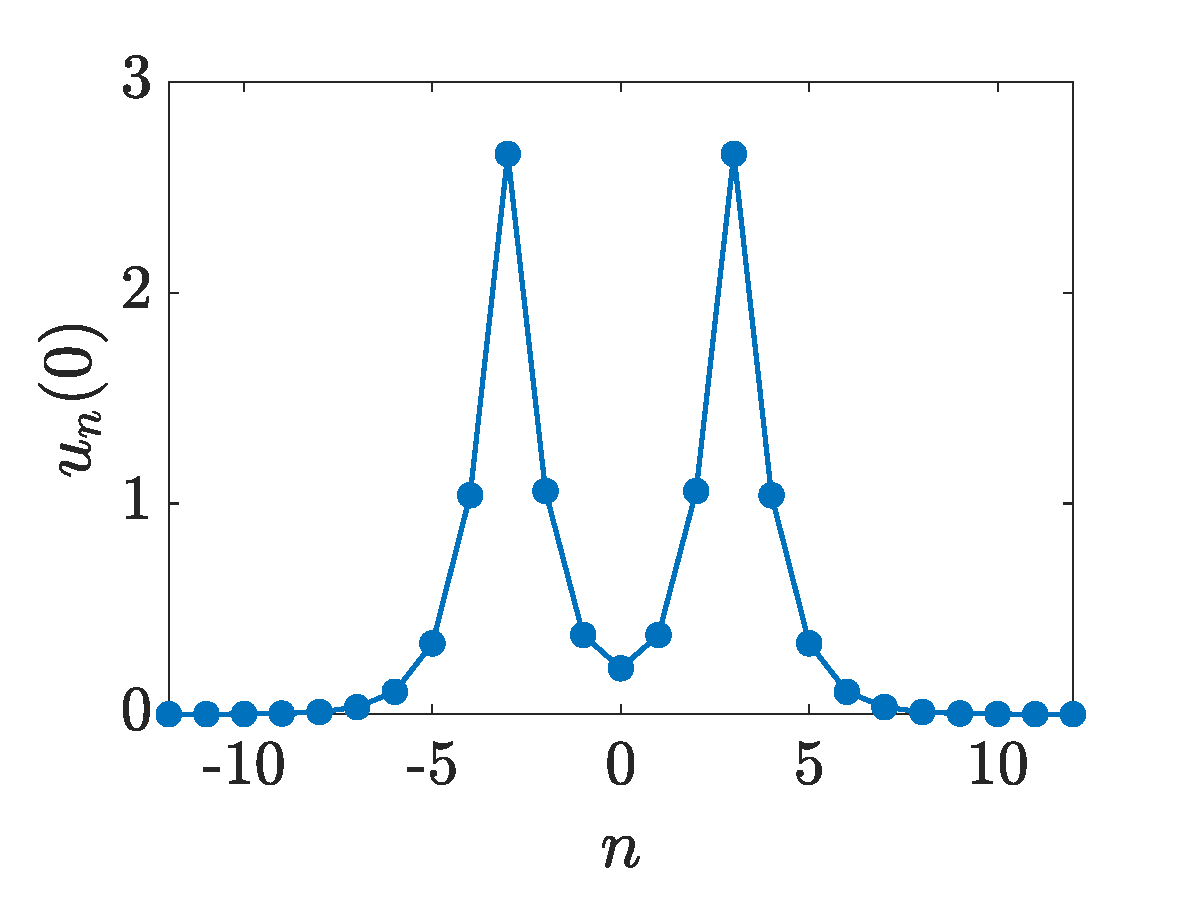
\includegraphics[width=5.5cm]{doubleppun0.eps} \hspace{-0.5cm}
	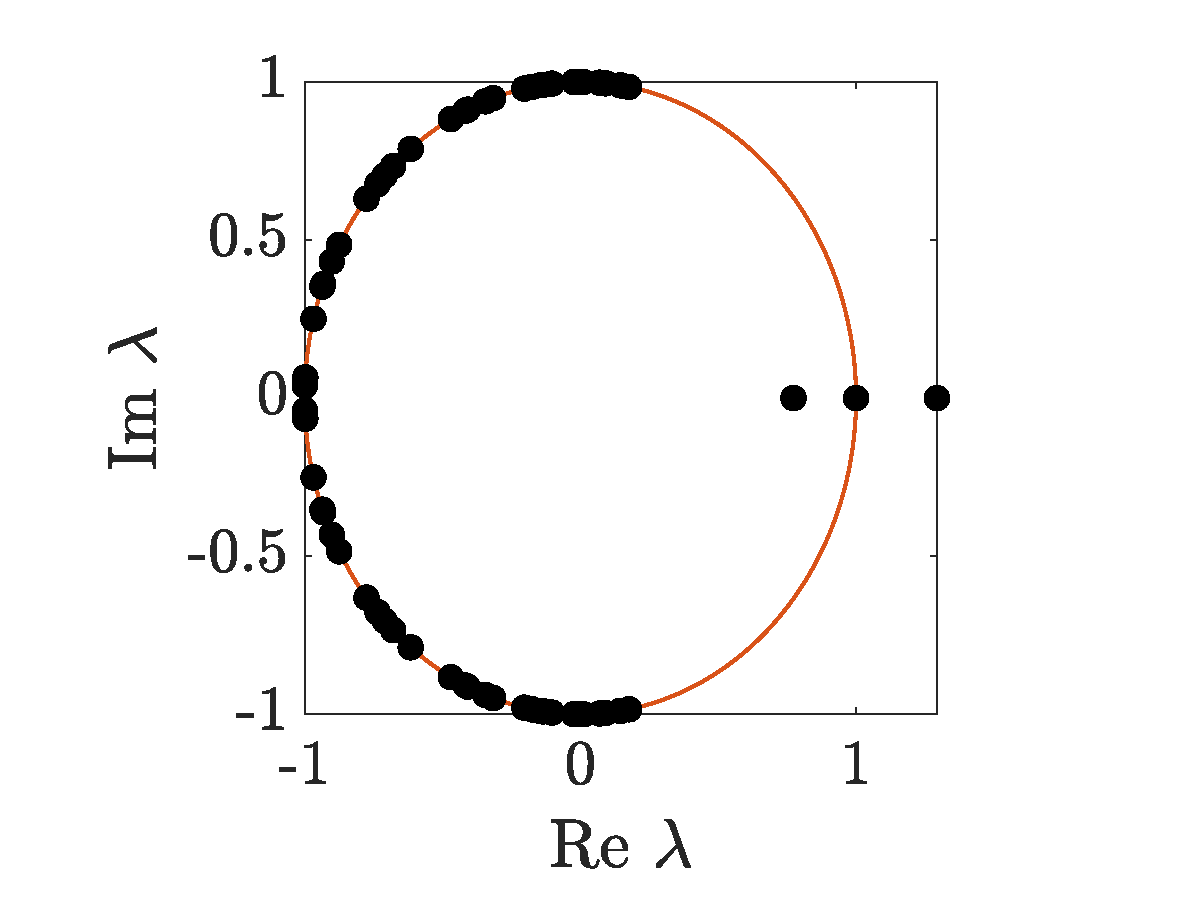
\includegraphics[width=5.5cm]{doubleppspec.eps} \hspace{-0.5cm}
	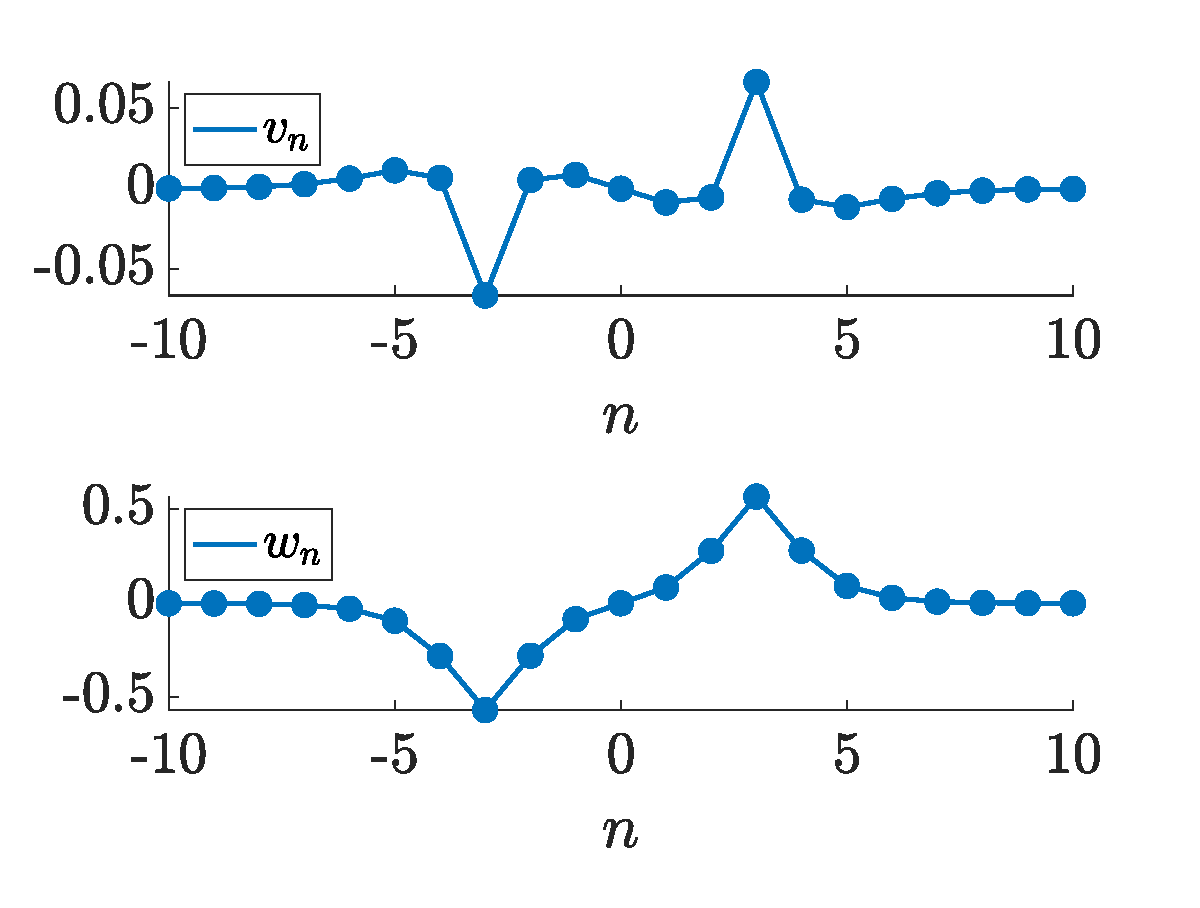
\includegraphics[width=5.5cm]{doubleppinteig.eps} 
	% \end{tabular}
	\end{center}
	\caption{Double}
	\label{fig:double}
\end{figure}

\begin{figure}
	\begin{center}
	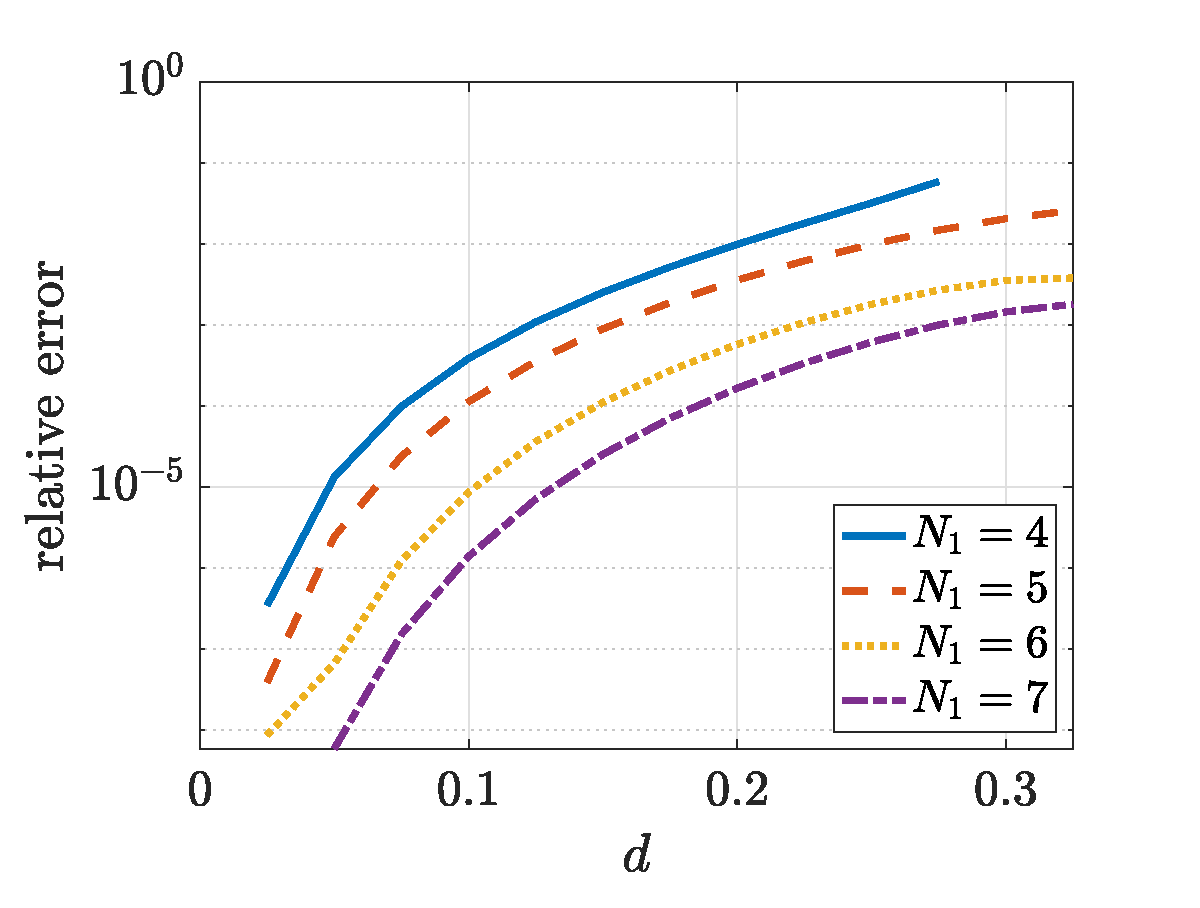
\includegraphics[width=5.5cm]{doubleeigerrord.eps} \hspace{-0.5cm}
	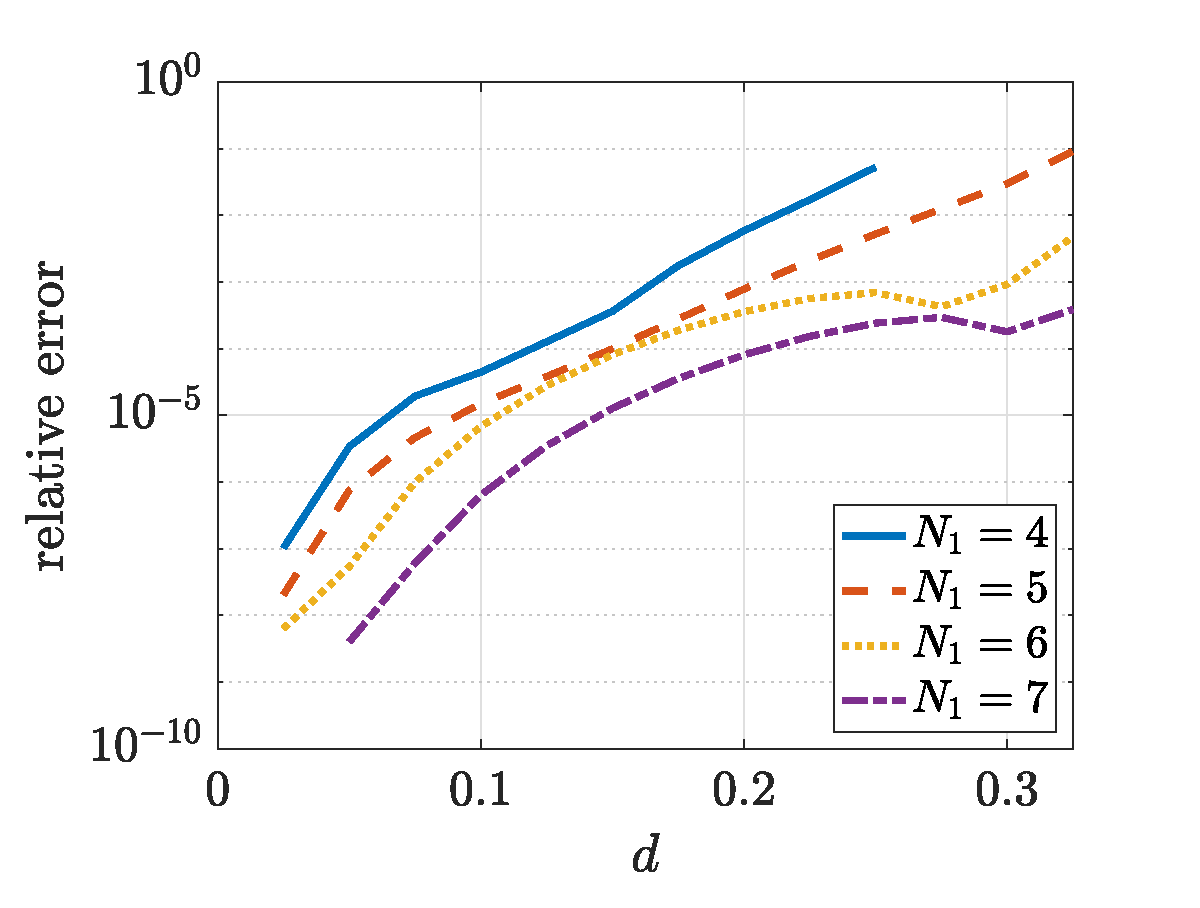
\includegraphics[width=5.5cm]{doubleppeigerrord.eps} \hspace{-0.5cm}
	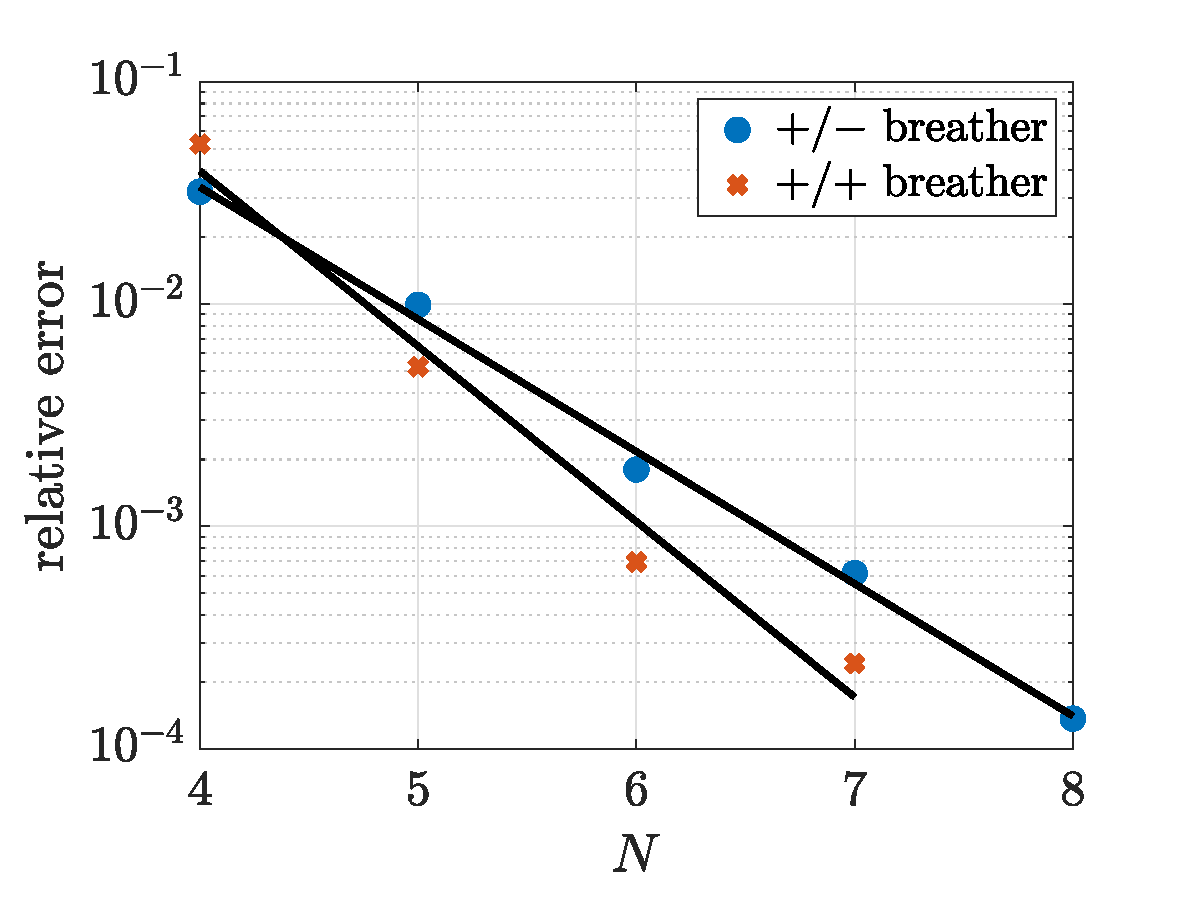
\includegraphics[width=5.5cm]{doubleeigerrorN.eps} 
	% \end{tabular}
	\end{center}
	\caption{Eigenvalue error plots}
	\label{fig:eigerror}
\end{figure}

\begin{figure}
	\begin{center}
	\begin{tabular}{cc}
	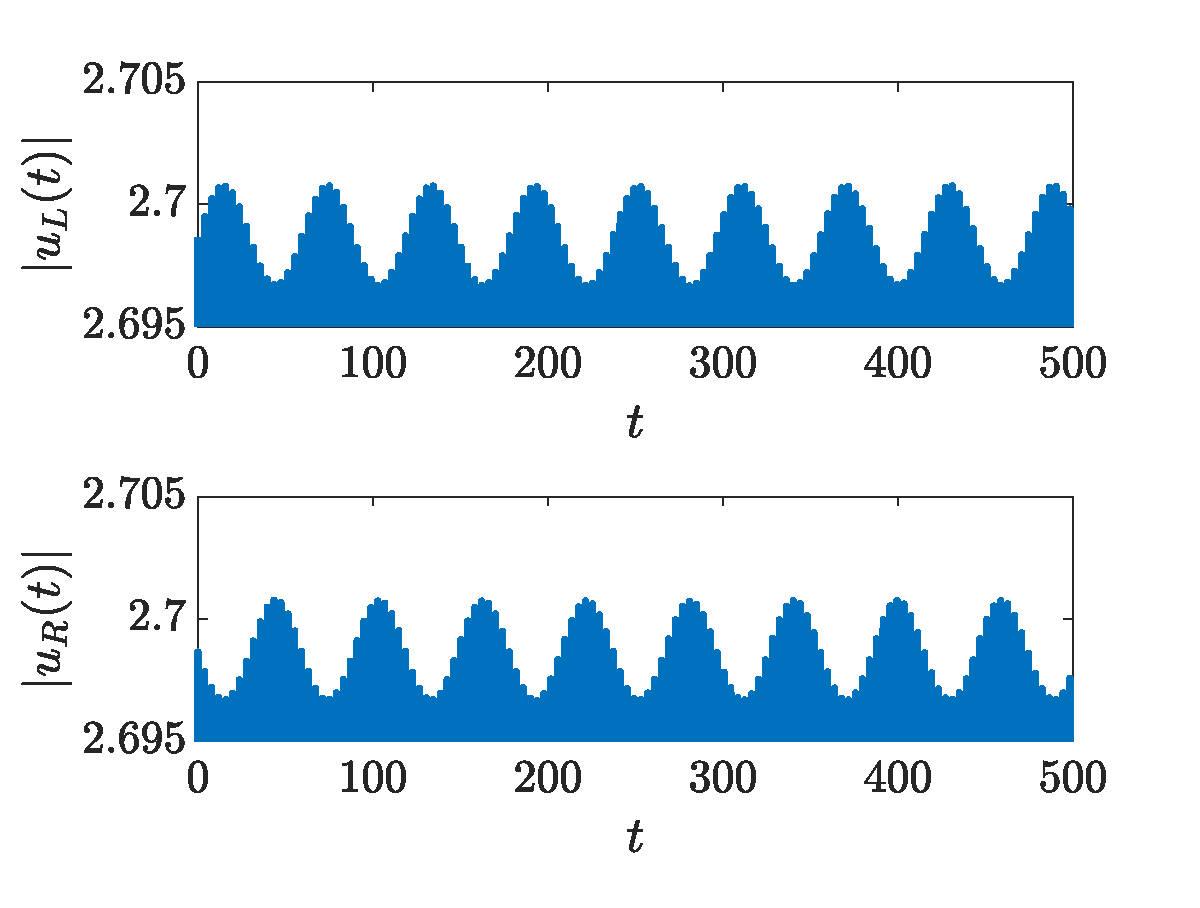
\includegraphics[width=7.5cm]{timestepN6.eps} &
	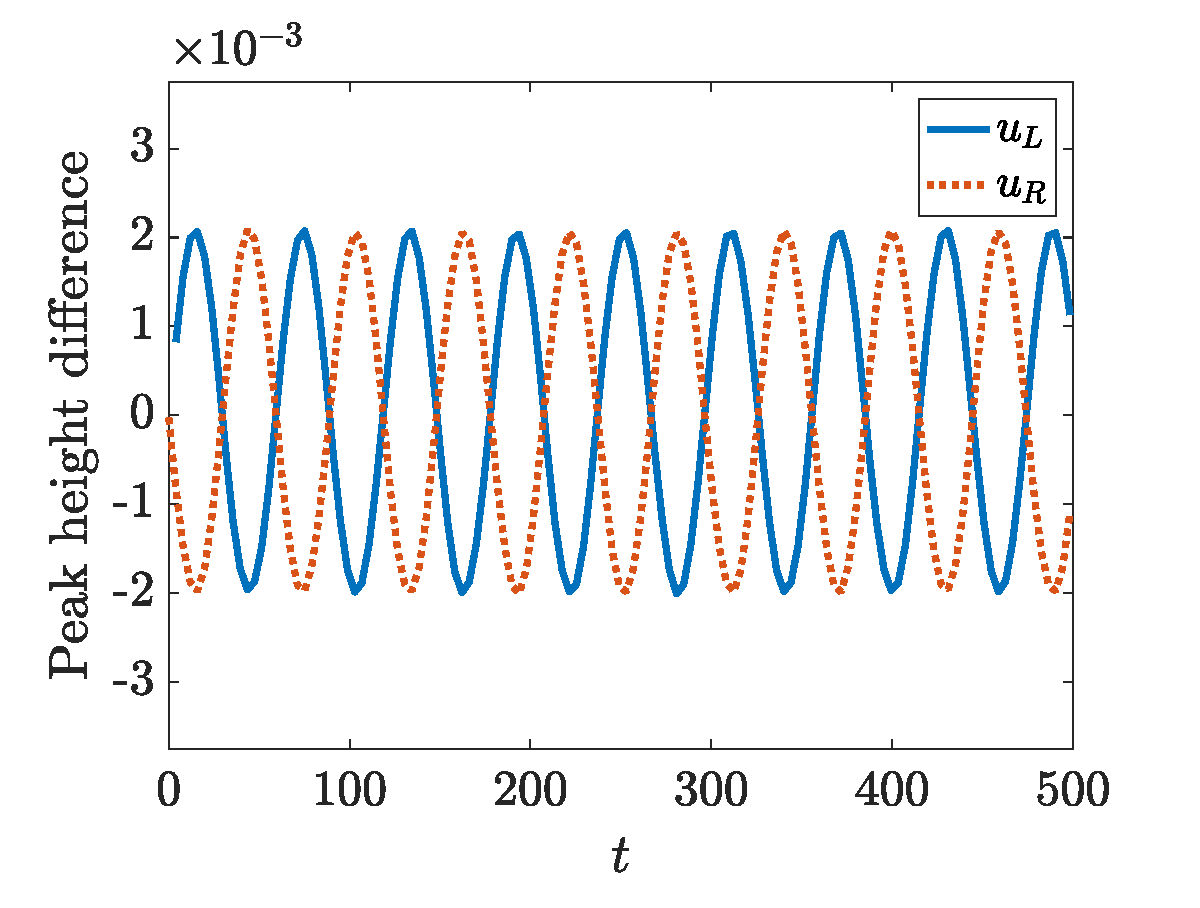
\includegraphics[width=7.5cm]{timestepN6pks.eps} \\ 
	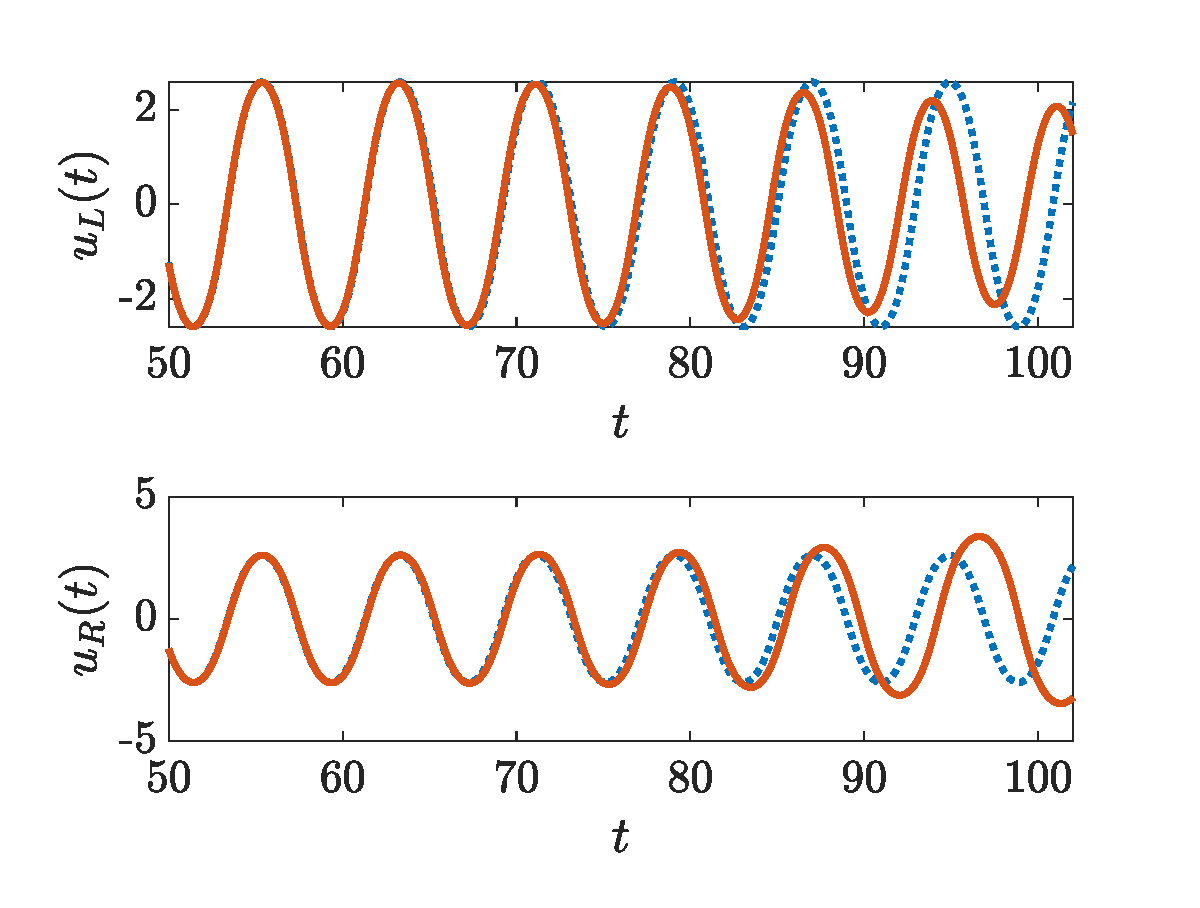
\includegraphics[width=7.5cm]{timestepN6pp.eps} &
	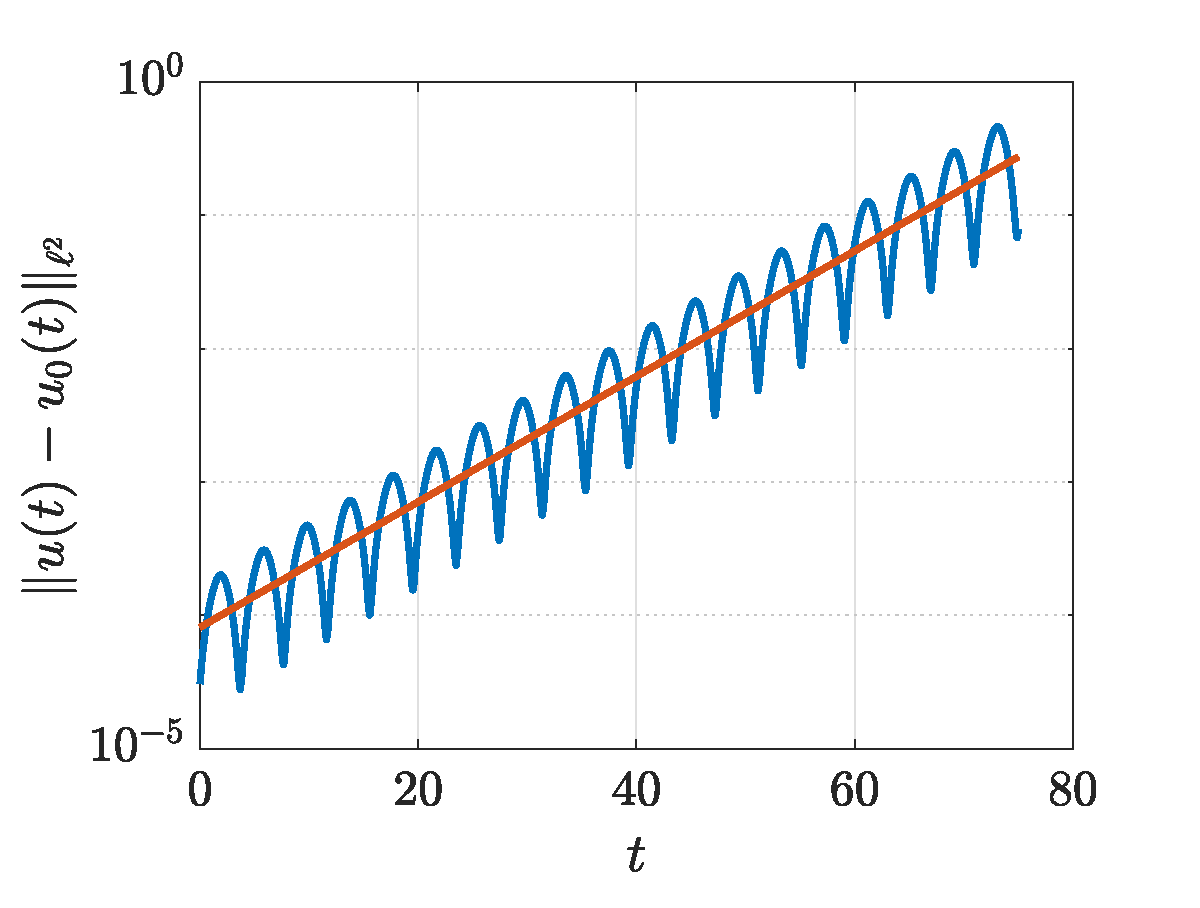
\includegraphics[width=7.5cm]{timestepN6growth.eps}
	\end{tabular}
	\end{center}
	\caption{Timestepping}
	\label{fig:timestepSG}
\end{figure}



\paragraph{Acknowledgments}

This material is based upon work supported by the U.S. National Science Foundation under the RTG grant DMS-1840260 (R.P. and A.A.)
and DMS-1809074 (P.G.K.).

\bibliographystyle{amsplain}
\bibliography{DKG.bib}

\end{document}